\documentclass[../notes.tex]{subfiles}

\pagestyle{main}
\renewcommand{\chaptermark}[1]{\markboth{\chaptername\ \thechapter\ (#1)}{}}
\setcounter{chapter}{5}

\begin{document}




\chapter{Import and Export}
\section{Organelles and Transport}
\begin{itemize}
    \item \marginnote{11/1:}Warm-up activity: Quiz questions.
    \item This class and next class: Protein localization mechanisms and inhibition.
    \item Think about\dots
    \begin{itemize}
        \item How a cell transports and localizes proteins;
        \item Mechanisms of preventing things from going where they should.
    \end{itemize}
    \item Indeed, some protein inhibitors work not by inactivating proteins but by making sure they don't get to the right place.
    \item \textbf{Chaperone}: A small molecule that allows a misfolded protein in the wrong place to fold and reach its site of action.
    \begin{itemize}
        \item These are promising new drugs.
        \item Example: There is a known risk gene for Parkinson's disease. A protein gets stuck in the ER. If there are small molecules you can use to get the protein to fold in the ER and be released, you win.
        \item Example: Cardiovascular disease. Most drugs fail clinical trials right at the last stage of testing because they cause something called \textbf{long QT syndrome}.
        \begin{itemize}
            \item Said drugs cause this syndrome by preventing ion channels from reaching the plasma membrane.
            \item Chaperones could potentially help overcome this common barrier.
        \end{itemize}
    \end{itemize}
    \item \textbf{Arrhythmia}: A fast, chaotic heartbeat.
    \item \textbf{Long QT syndrome}: A heart signaling disorder that can cause arrhythmias.
    \begin{itemize}
        \item Symptoms can be severe, up to death.
    \end{itemize}
    \item Today: Mechanisms of protein localization.
    \begin{itemize}
        \item How do proteins reach the nucleus, mitochondria, and a mystery organelle? These are open questions in basic biology.
    \end{itemize}
    \item Organelles and membranes by the numbers.
    \begin{itemize}
        \item Cytosol: 2\% of the membrane in a cell, but 54\% of total cell volume.
        \item Thus, the plasma membrane spends a lot of energy keeping the cytosol happy.
        \item The mitochondria and ER have a huge amount of membrane but very little volume and contribute to keeping the cytosol happy as well.
        \begin{itemize}
            \item The membrane content helps maintain homeostasis.
        \end{itemize}
        \item What was the net point of all this??
    \end{itemize}
    \item Evolution of compartments.
    \begin{itemize}
        \item Helps us understand \textbf{topological equivalence}.
        \item Yamuna believes that the endosymbiotic theory is just a hypothesis and that it's all up in the air and likely to change.
        \item Current hypothesis: Archaea lost its cell wall making it easier for it to acquire DNA. Once it acquired enough valuable genes, the cell membrane underwent an invagination to form the nucleus and extra folds of the ER. This prevents the cell from losing the DNA its acquired.
        \begin{itemize}
            \item This is why the ER and extracellular matrix are topologically equivalent, i.e., because the former evolved from the latter.
        \end{itemize}
        \item Mitochondria are the cell intaking another bacteria that could produce energy.
    \end{itemize}
    \item \textbf{Topologically equivalent} (compartments): Two compartments inside (or outside) a cell such that materials do not have to cross a membrane to get from one to the other.
    \begin{figure}[h!]
        \centering
        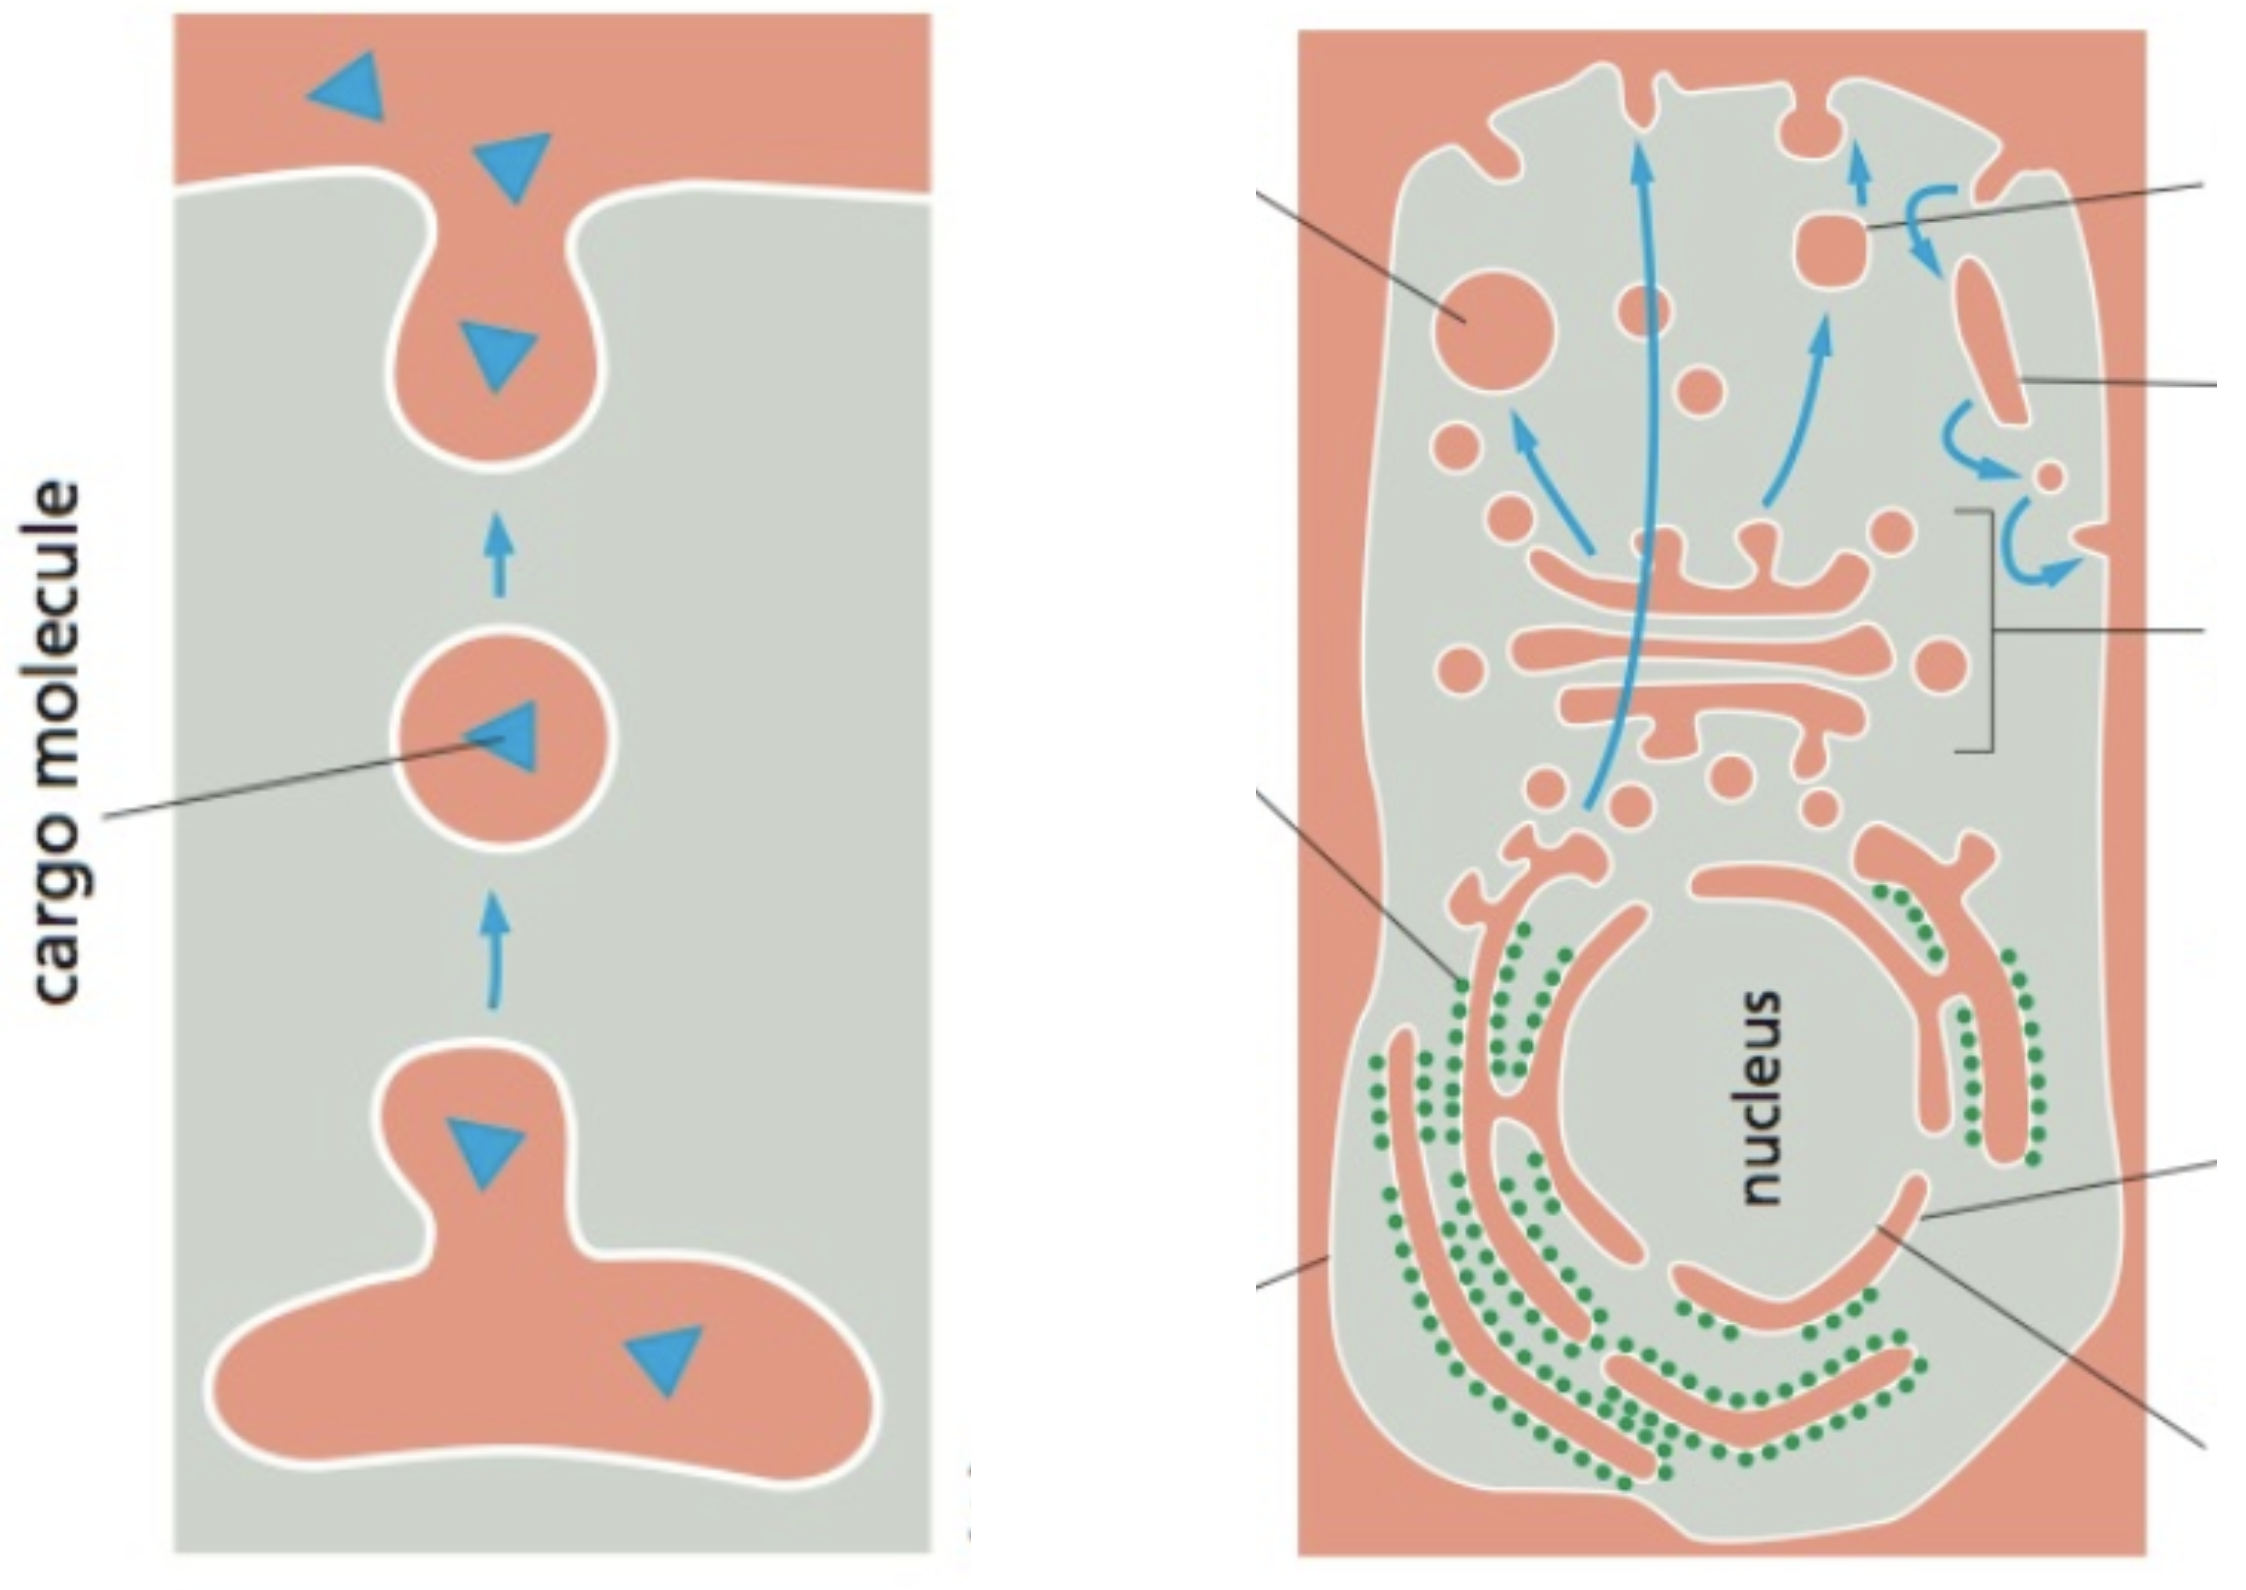
\includegraphics[width=0.4\linewidth]{../ExtFiles/topologicalEquivalence.png}
        \caption{Topological equivalence.}
        \label{fig:topologicalEquivalence}
    \end{figure}
    \begin{itemize}
        \item Example: Golgi and ER are topologically equivalent (and topologically equivalent to the extracellular matrix) but not to the cytoplasm. This is because materials in the ER move to the Golgi and then to the extracellular matrix within a \textbf{vesicle}, i.e., they never have to cross a plasma membrane so much as they get surrounded and moved by different membranes.
        \item Example: The extracellular matrix and the cytoplasm are not topologically equivalent. Notice that any material coming into the cytoplasm from the outside must cross through the plasma membrane using one of the mechanisms from last class (we're not talking endocytosis yet).
    \end{itemize}
    \item Proteins can be transported between organelles either by being stuck in the membrane of a vesicle (at which point they will end up in the membrane of the target organelle) or within said vesicle's lumen (at which point they will end up in the lumen of the target organelle).
    \item Isolating organelles.
    \begin{figure}[h!]
        \centering
        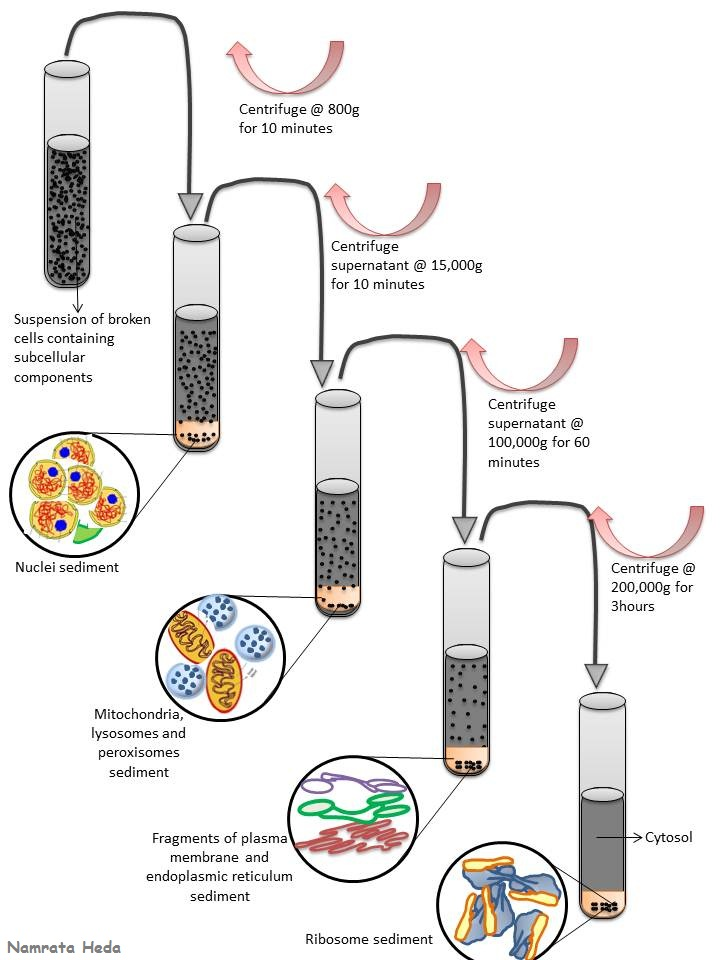
\includegraphics[width=0.5\linewidth]{../ExtFiles/isolatingOrganelles.jpeg}
        \caption{Isolating organelles.}
        \label{fig:isolatingOrganelles}
    \end{figure}
    \begin{itemize}
        \item We discover transport mechanisms by carrying out a lot of mutations and then isolating specific target organelles and testing for a protein's presence (look for a ratio between the quantity of this protein present and a standard protein that you know will be there).
        \item Isolation mechanism: We take a bunch of cells, dissolve the extracellular membrane to get a soup of organelles, centrifuge it (to let heavy organelles like the nucleus fall out), centrifuge again (to get the small organelles like the mitochondria, lysosomes, and peroxisomes), centrifuge it again (to get fragments of the plasma membrane and ER), and centrifuge it one last time (to get ribosomes).
        \item Alternative isolation mechanism: Use a matrix with a density gradient and just centrifuge once to get multiple layers.
    \end{itemize}
    \item Three main ways to move proteins in a cell.
    \begin{itemize}
        \item Recall passive and active exchange.
        \item You can let physical equilibrium take hold, of course, but often that won't lead to great enough concentrations.
        \item Thus, cells evolved the following three methods\dots
    \end{itemize}
    \item \textbf{Gated transport}: A type of transport involving a gate and a condition (e.g., a binding or membrane potential) that must be satisfied for the gate to "lift open."
    \item \textbf{Translocation}: The movement between topologically nonequivalent compartment.
    \begin{itemize}
        \item Example: Suppose you have a protein that's been made in the ER, has been deposited into the cytoplasm, and now needs to get into the mitochondria. We will consider this example in much greater detail shortly.
    \end{itemize}
    \item \textbf{Vesicular transport}: The movement of biomolecules in vesicles between topologically equivalent compartments.
    \item \textbf{Localization sequence}: A molecular GPS. \emph{Also known as} \textbf{nuclear localization sequence}, \textbf{NLS}.
    \begin{itemize}
        \item Usually located on the N-terminus because it comes out first and needs to know where to go.
        \item Localization sequences have different strengths. Some send proteins in a high fraction somewhere; some send proteins in a low fraction somewhere.
        \begin{itemize}
            \item Strength is determined by the sequence's affinity for the transport protein. We will discuss this in more depth later.
        \end{itemize}
        \item Length: Tetrapeptides up to 20-30 AAs.
        \item Very occasionally occur in the middle of a protein.
    \end{itemize}
    \item \textbf{Translocation sequence}: A molecular GPS on the C-terminus that moves a protein after folding.
    \item Gated transport example: Movement from the cytosol into the nucleus.
    \begin{itemize}
        \item This is also the most common type of gated transport.
        \item The gate is the nuclear pore, and the condition is \textbf{karyopherin} binding
    \end{itemize}
    \item \textbf{Karyopherin}: A protein involved in transporting molecules between the cytoplasm and the nucleus.
    \item Consider first the structure of the \textbf{nuclear pores}.
    \item \textbf{Nuclear pore}: A gateway from the cytosol to the nucleus.
    \begin{figure}[h!]
        \centering
        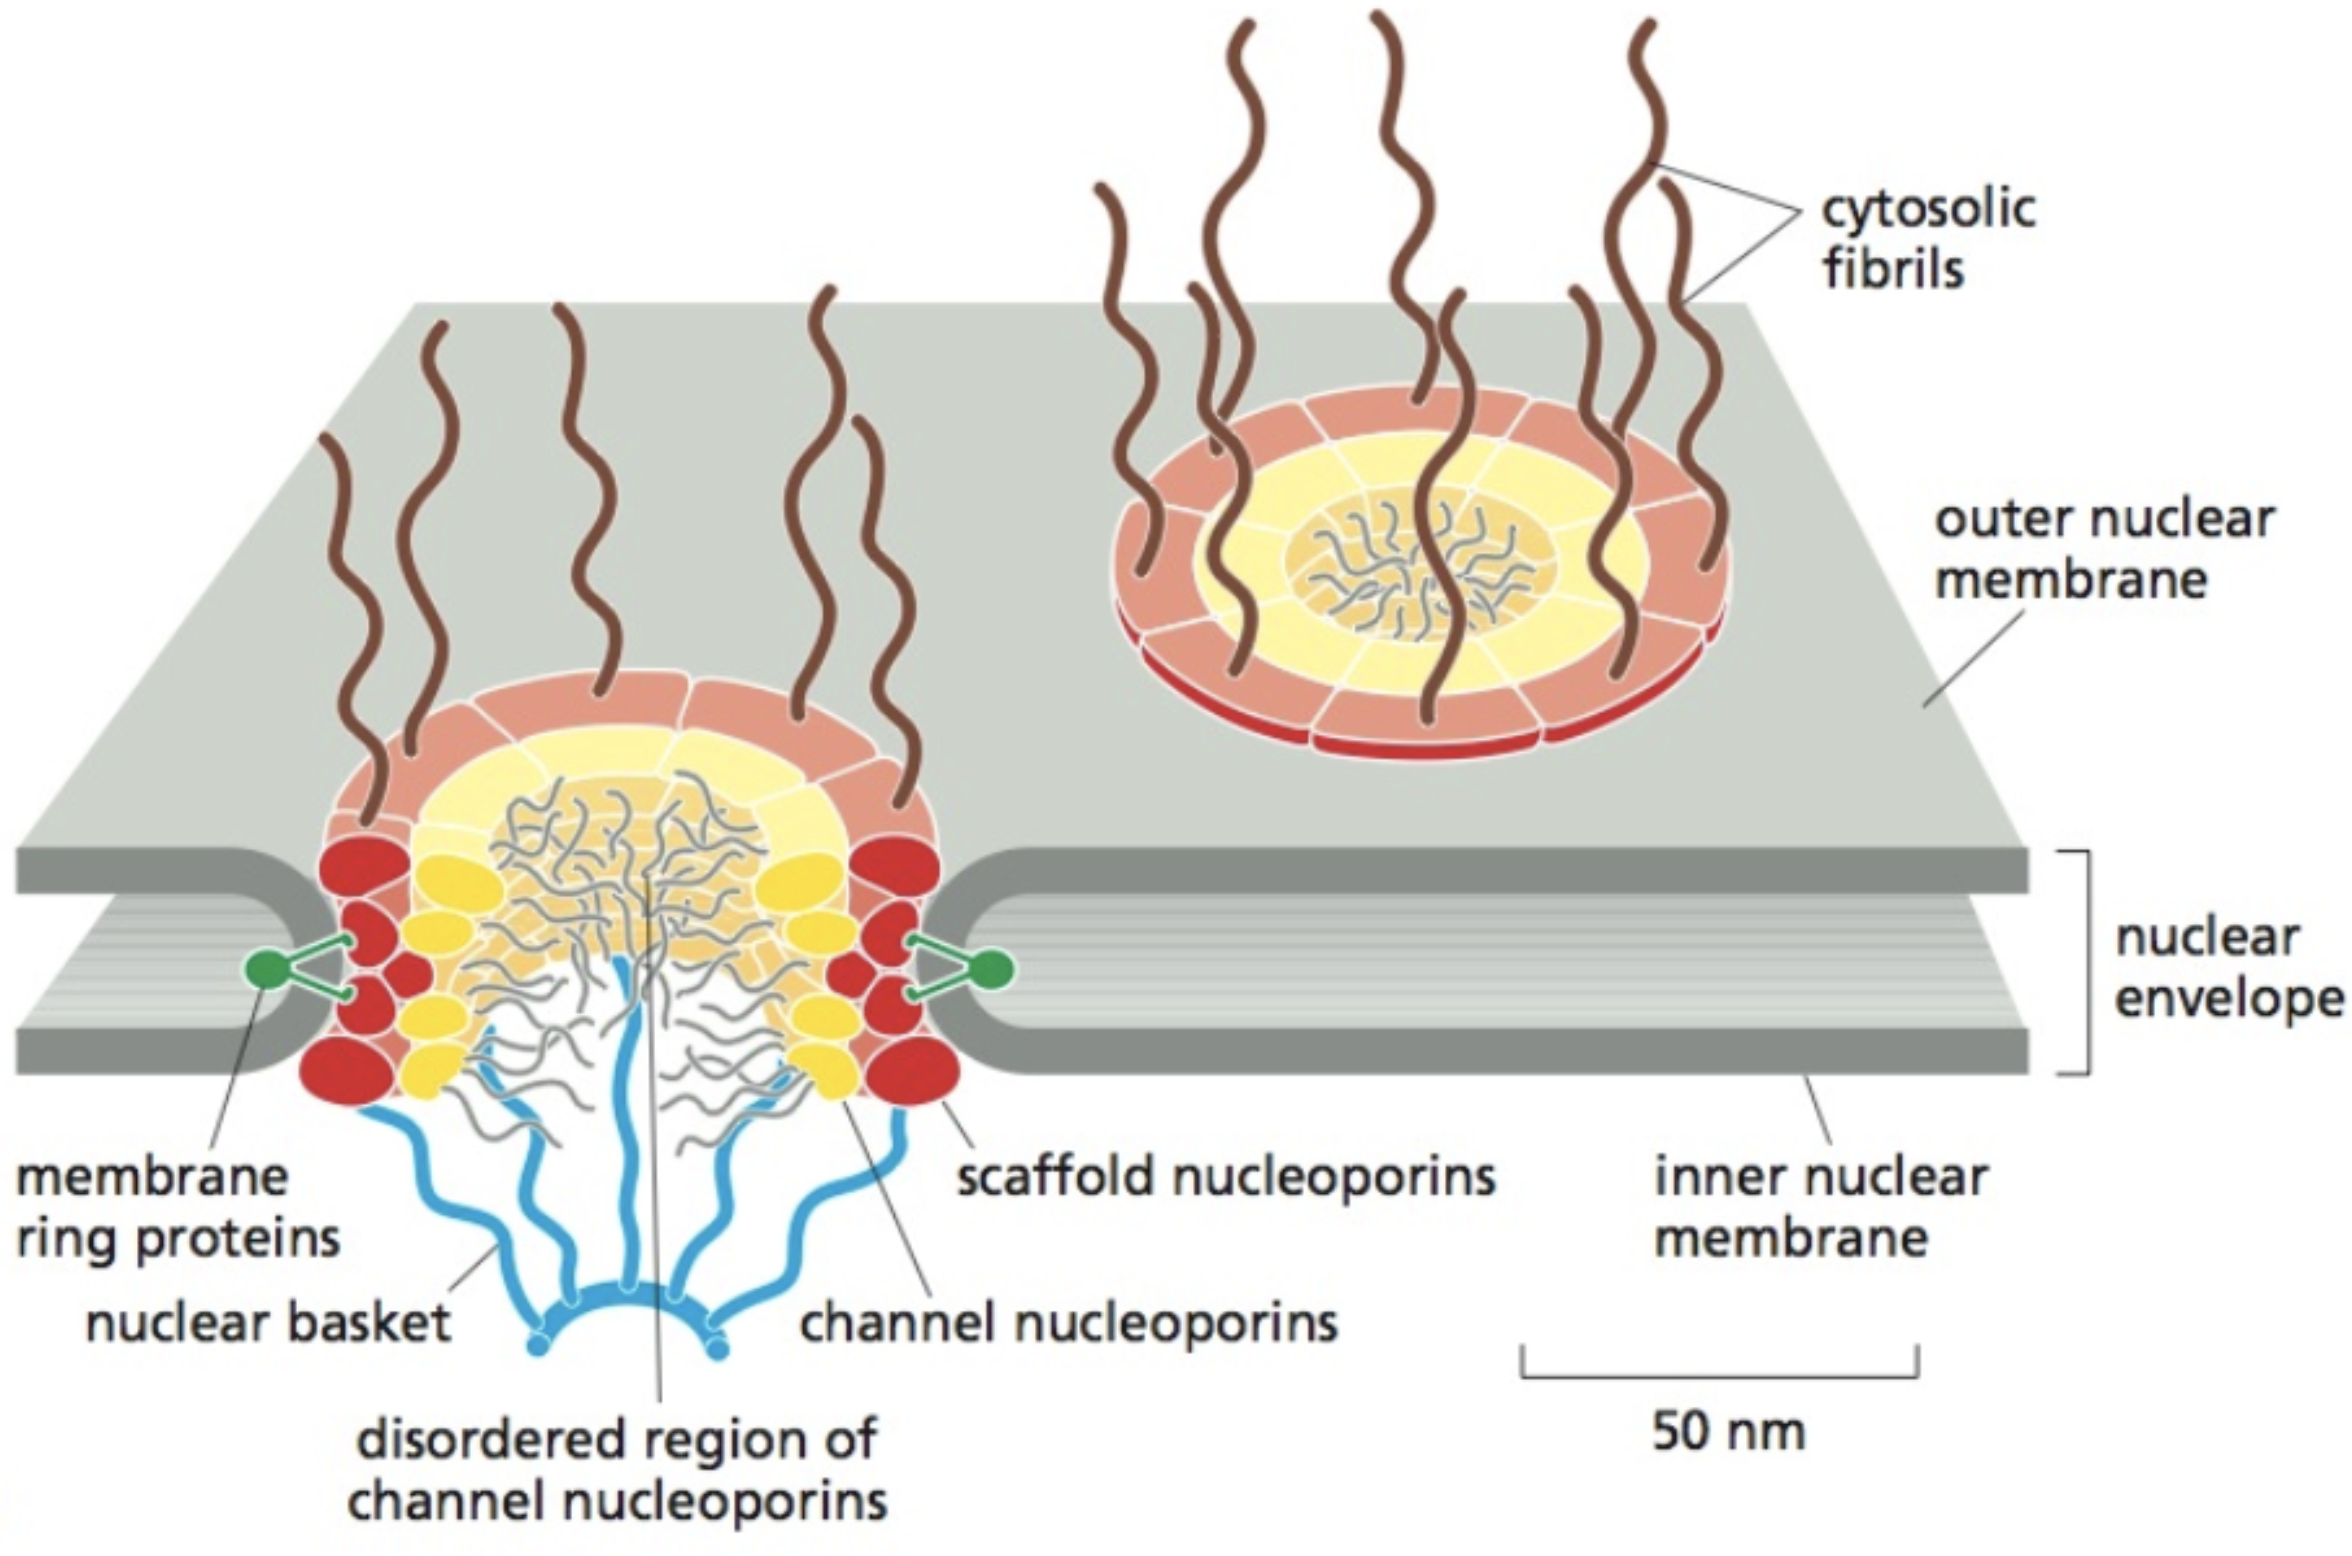
\includegraphics[width=0.5\linewidth]{../ExtFiles/nuclearPore.png}
        \caption{Nuclear pore structure.}
        \label{fig:nuclearPore}
    \end{figure}
    \begin{itemize}
        \item Nuclei have double plasma membranes and nuclear pores. All transport in and out of the nucleus occurs via nuclear pores.
        \item \textbf{Membrane ring proteins} make the membrane bend backward around nuclear pores.
        \item There are about 3000 nuclear pores per nucleus.
        \item About 1000 molecules transport both ways per nuclear pore per second.
        \item Active v. passive transport: Anything smaller than \SI{40}{\nano\meter} will freely diffuse to a significant extent (smaller implies higher passive transport). Larger, you need something to capture it and drag it through (this is active transport).
        \item Nuclear pores are 8-fold symmetric bodies.
        \begin{itemize}
            \item We still don't know the complete structure.
            \item Composed of \textbf{nucleoporins}.
            \item Hair-like \textbf{cytosolic fibrils} on the outside and a \textbf{nuclear basket} on the inside.
            \item A porous plug in the center; still don't know what it is, but it's made of lots of FG repeats.
        \end{itemize}
    \end{itemize}
    \item \textbf{Nucleoporin}: A protein that is a constituent building block of the nuclear pore complex. \emph{Also known as} \textbf{nap}.
    \begin{itemize}
        \item There are permanent naps, but there are also naps which come off and on.
        \item Approximately 30 exist.
        \item Some are transmembrane.
    \end{itemize}
    \item Probing NLS-enabled nuclear import.
    \begin{figure}[H]
        \centering
        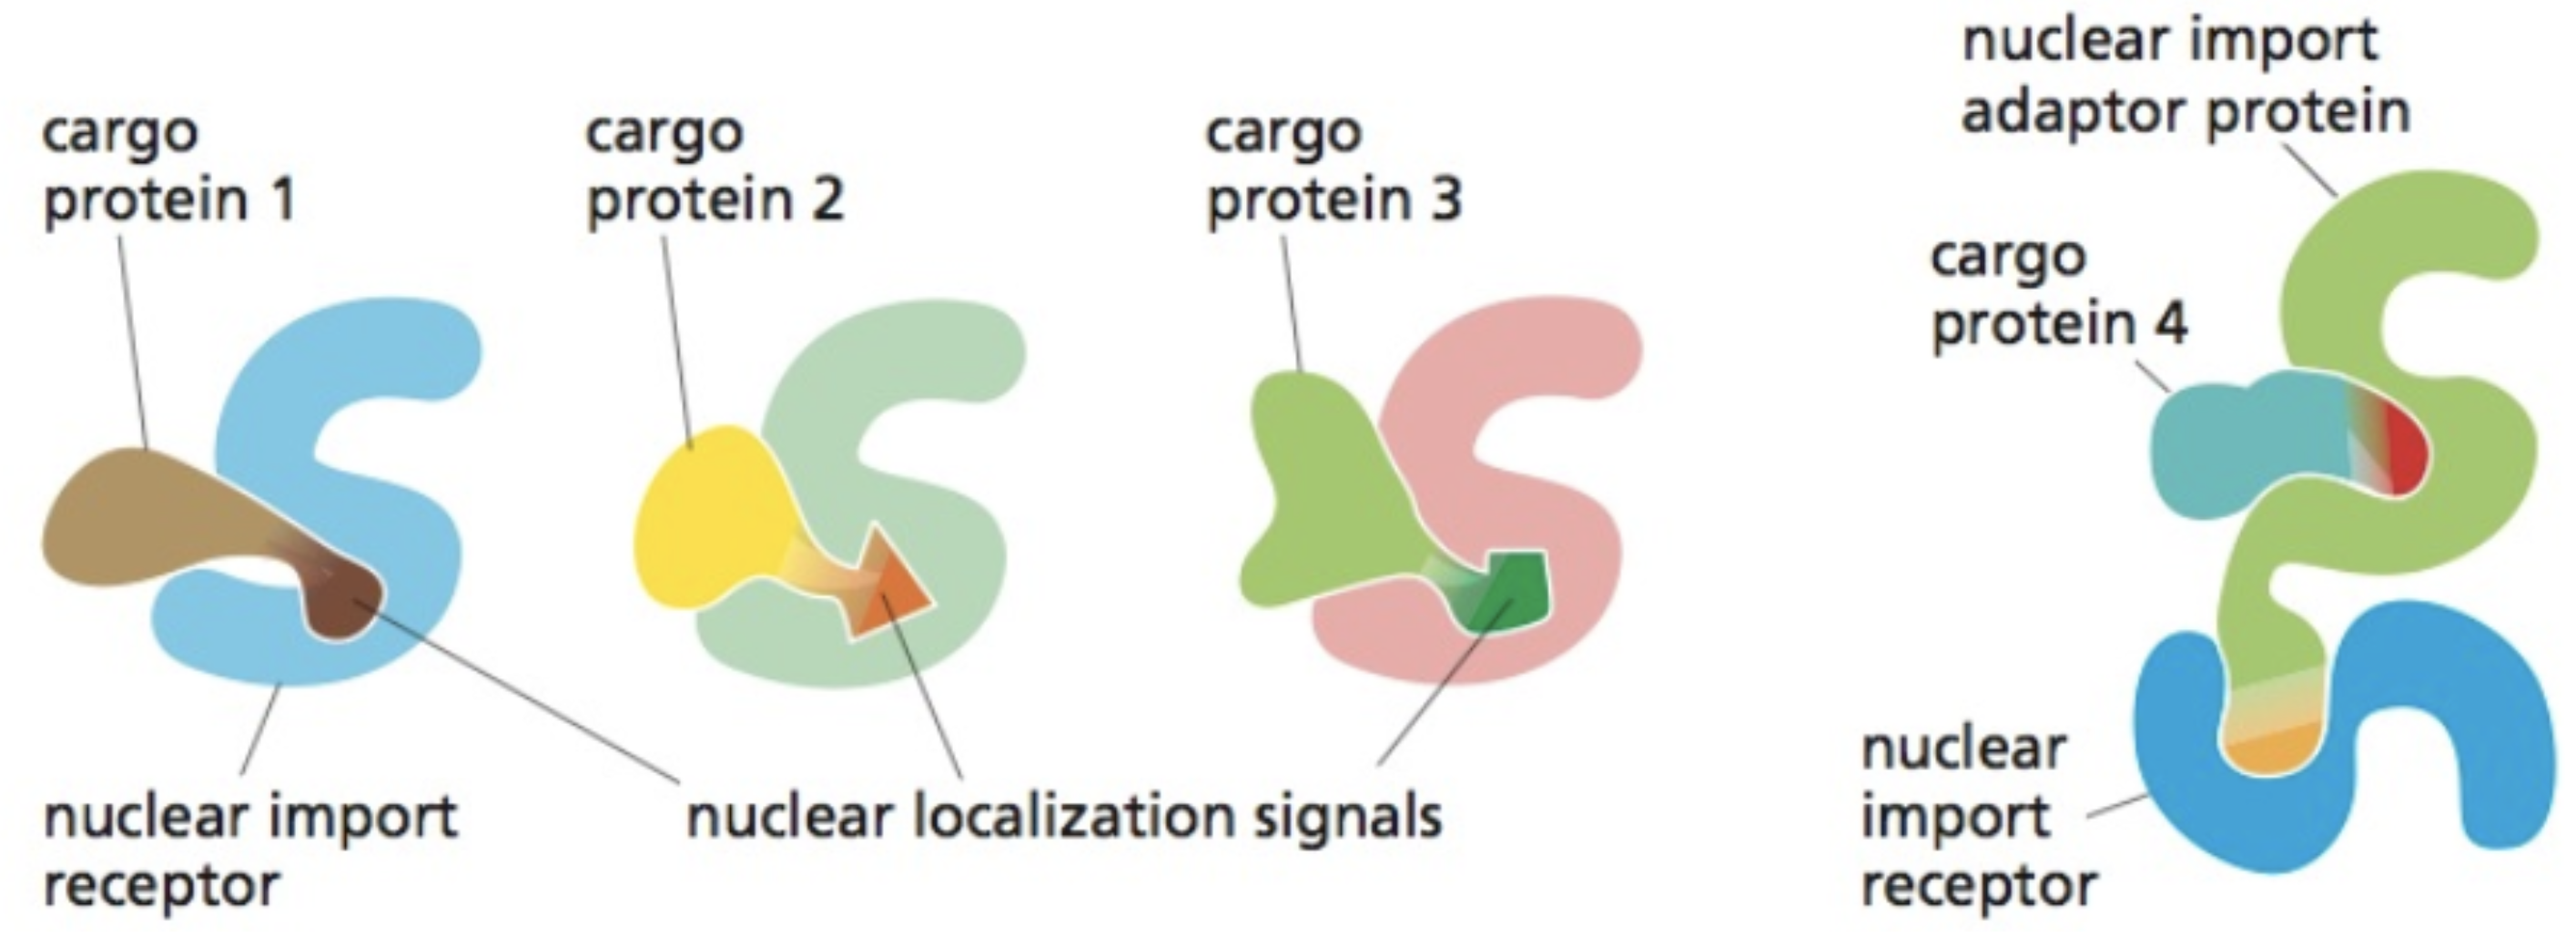
\includegraphics[width=0.5\linewidth]{../ExtFiles/NLSimport.png}
        \caption{Nuclear import receptor binding.}
        \label{fig:NLSimport}
    \end{figure}
    \begin{itemize}
        \item Suppose we fuse an NLS with GFP (for which a Nobel Prize has been awarded).
        \item If, in the NLS sequence, we change a $\text{K}\to\text{T}$, then localization of the sequence is significantly decreased.
        \begin{itemize}
            \item Review: Replacing positively charged lysine with polar threonine would certainly affect the interaction between the NLS and the \textbf{nuclear import receptor}!
        \end{itemize}
        \item Conclusion: We can affect NLS efficiency by altering one's affinity for its karyopherin (or vice versa), or by altering the ability of the karyopherin to enter the nucleus.
        \item "It depends upon which bus you get on and upon the strength of your ticket."
        \item Benefit of differential binding affinities: It is possible to have different concentrations of different proteins. You don't want all proteins in the nucleus to have the same concentration, after all.
        \item There also exist \textbf{nuclear import adaptor proteins} which link cargo proteins to their nuclear import receptors with higher binding affinities.
    \end{itemize}
    \item Nuclear export is the reverse of nuclear import.
    \begin{itemize}
        \item Before we can discuss nuclear export directly, we should discuss the Ran proteins.
        \begin{figure}[h!]
            \centering
            \begin{subfigure}[b]{0.49\linewidth}
                \centering
                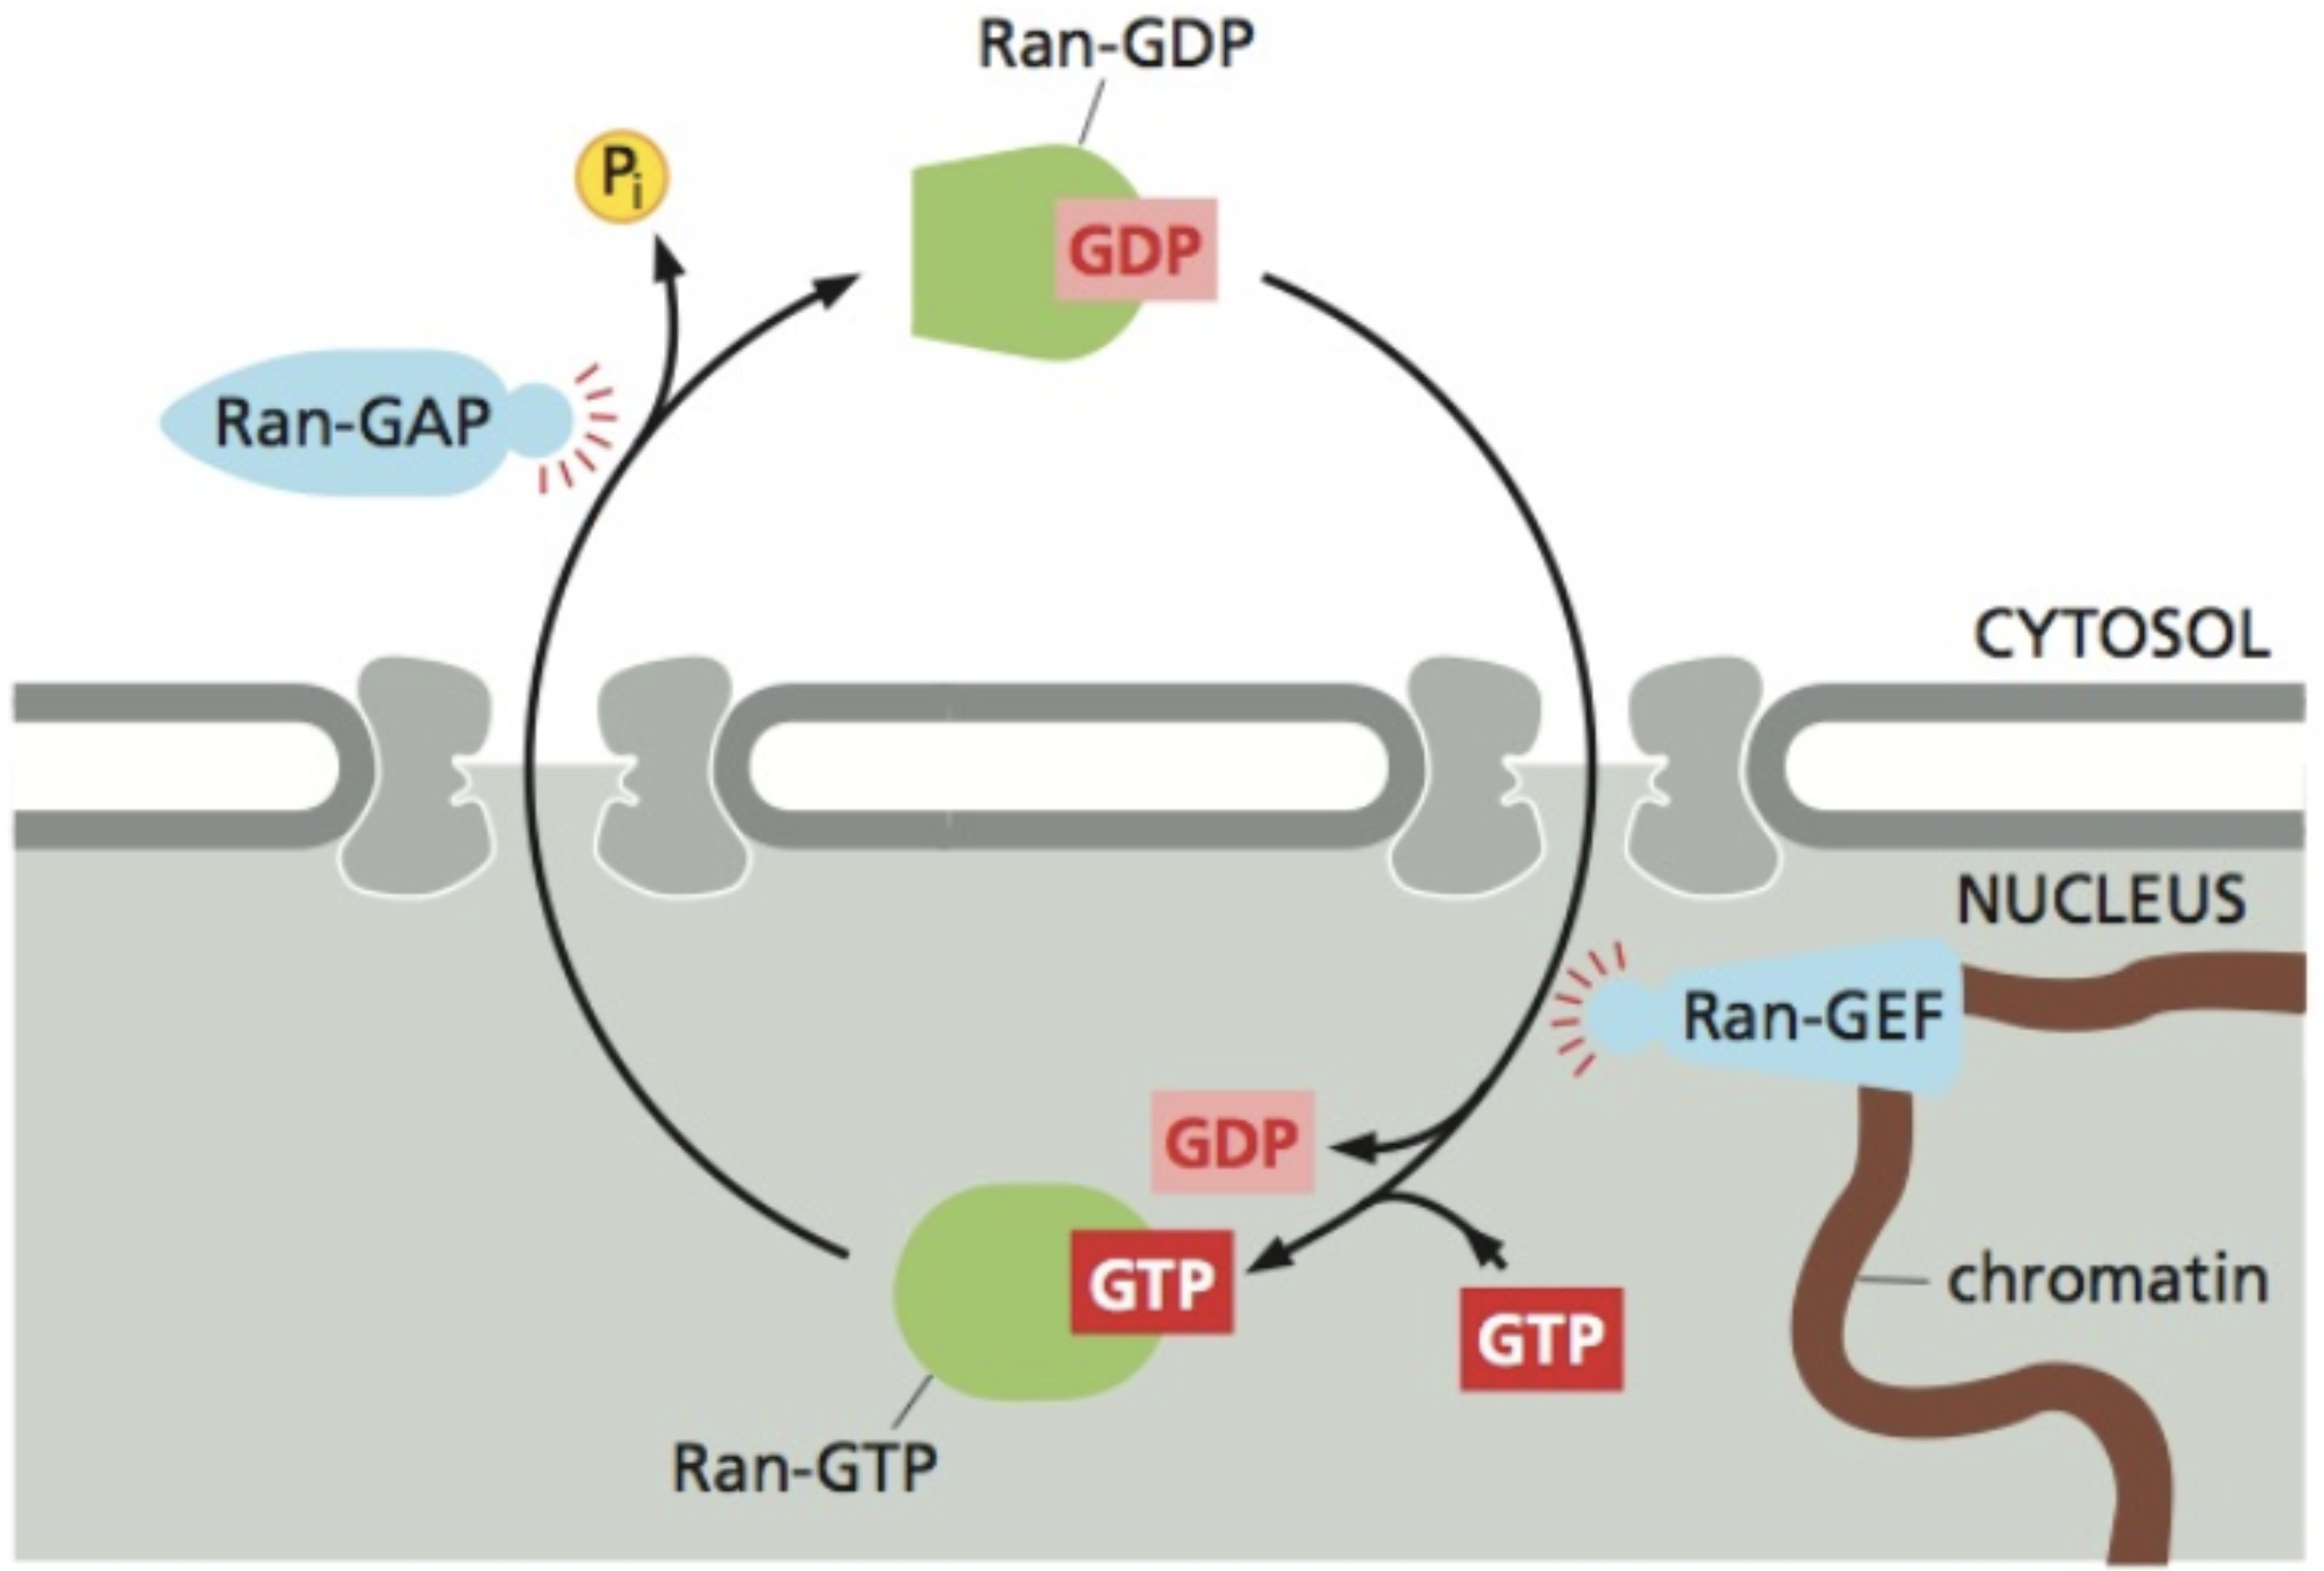
\includegraphics[width=0.8\linewidth]{../ExtFiles/nuclearImpExpa.png}
                \caption{The Ran proteins.}
                \label{fig:nuclearImpExpa}
            \end{subfigure}
            \caption{Nuclear import and export mechanism.}
        \end{figure}
        \begin{itemize}
            \item Ran complexes have a domain called a \textbf{GTPase domain}.
            \item Ran's GTPase domain has GTP- and GDP-bound forms.
            \item There is a Ran-GDP / Ran-GTP gradient across the nuclear membrane: Ran-GTP is present in much higher concentrations within the nucleus, and Ran-GDP is present in much higher concentrations outside the nucleus.
            \item Ran-GAP is a \textbf{GAP} for Ran-GTP and Ran-GEF is a \textbf{GEF} for Ran-GDP.
            \item Ran-GAP is localized in the cytosol, and Ran-GEF is localized in the nucleus (it sits on chromatin inside the nucleus).
        \end{itemize}
        \item We are now ready to discuss nuclear import and export.
        \begin{figure}[h!]
            \ContinuedFloat
            \centering
            \begin{subfigure}[b]{0.49\linewidth}
                \centering
                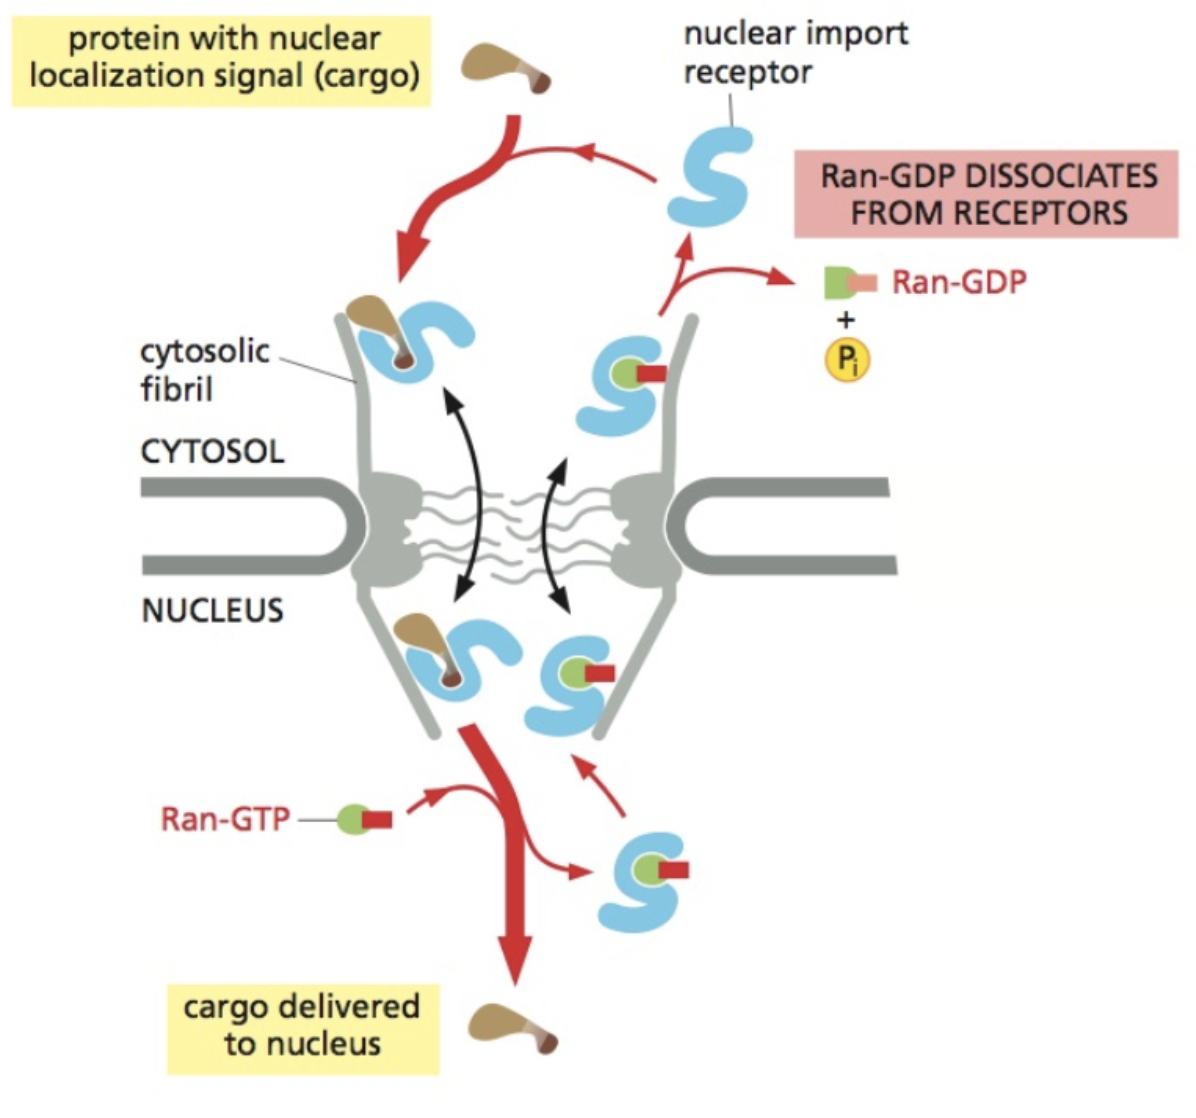
\includegraphics[width=0.82\linewidth]{../ExtFiles/nuclearImpExpb.png}
                \caption{Nuclear import.}
                \label{fig:nuclearImpExpb}
            \end{subfigure}
            \begin{subfigure}[b]{0.49\linewidth}
                \centering
                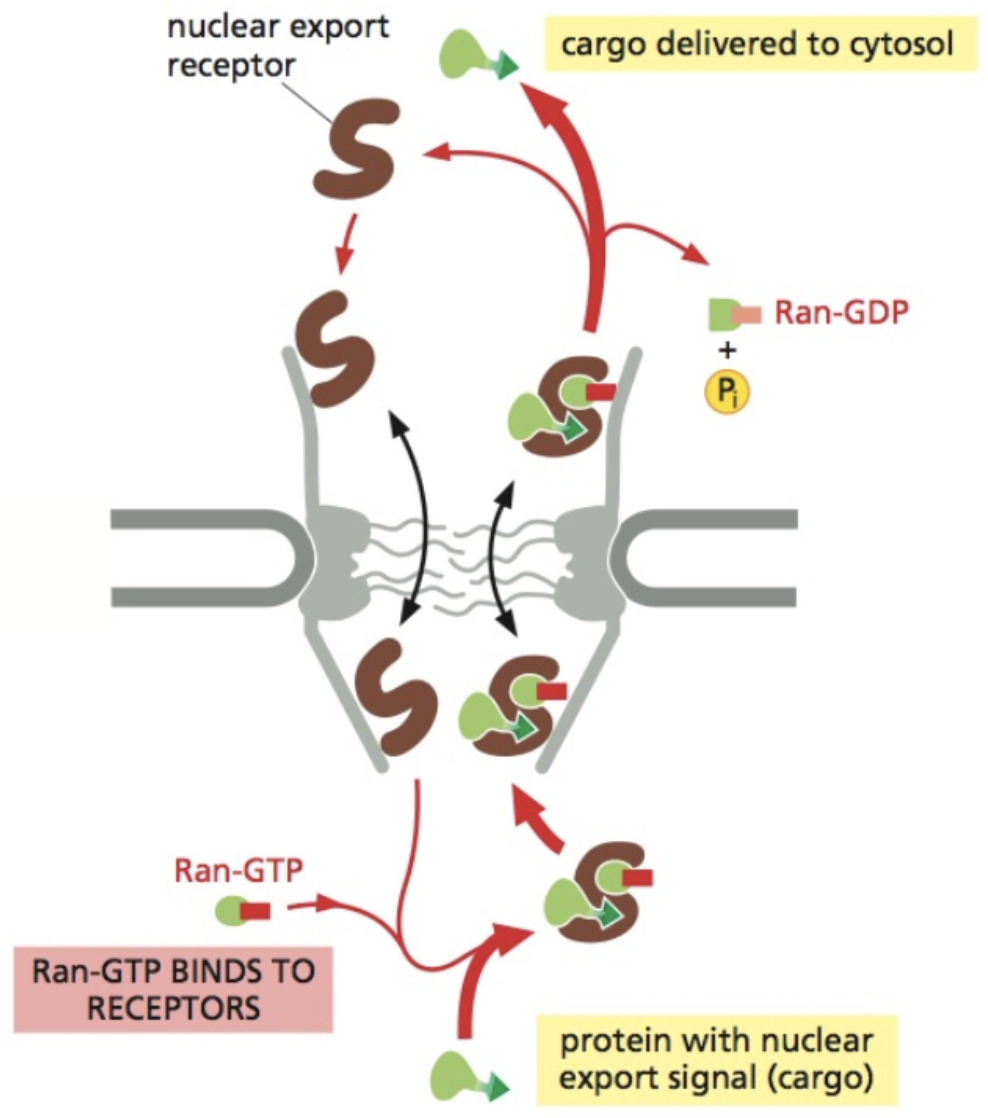
\includegraphics[width=0.7\linewidth]{../ExtFiles/nuclearImpExpc.png}
                \caption{Nuclear export.}
                \label{fig:nuclearImpExpc}
            \end{subfigure}
            \caption{Nuclear import and export mechanism.}
            \label{fig:nuclearImpExp}
        \end{figure}
        \begin{itemize}
            \item Nuclear importers first bind their proteins. Their hydrophobic regions are then caught by the cytosolic fibrils. Moving downward into the FG repeats, the importer's movement once inside is a random walk.
            \item Once an importer arrives in the nucleus, Ran-GTP attacks. Ran-GTP has a higher affinity for it than its substrate, so it will bind and cause the substrate to fall off, completing delivery to the nucleus.
            \item When the Ran-GTP-bound importer diffuses back out of the nucleus, Ran-GAP promotes GDP hydrolysis, and Ran-GDP dissociates.
            \item Nuclear export receptors random walk into the nucleus, bind a Ran-GTP, engage the cargo, random walk out of the nucleus, Ran-GAP hydrolyzes Ran-GTP to RanGDP which leaves, and this kicks out the cargo.
        \end{itemize}
        \item Note that as we would expect for an example of gated transport, a condition is met and only then does transport occur.
    \end{itemize}
    \item \textbf{GTPase domain}: A region of a protein that hydrolyzes a GTP to release energy, accelerating and powering the function of the protein.
    \begin{itemize}
        \item Carried by many kinds of proteins and is very powerful.
        \item Can help a ribozome work, help proteins move from the nucleus to the cytosol, promote vesicle fusing, etc.
        \item Essentially functions as a backpack with a battery.
    \end{itemize}
    \item \textbf{GAP}: A protein that promotes GTP hydrolysis in a GTPase domain that's already bound to GTP. \emph{Also known as} \textbf{GTPase activating protein}.
    \item \textbf{GEF}: A protein that exchanges GDP for GTP at the GTPase domain. \emph{Also known as} \textbf{Guanine nucleotide exchange factor}.
    \item Translocation example: Movement from the cytosol into a mitochondrion.
    \begin{itemize}
        \item Mitochondria have proteins that sit specifically on the outer membrane, inner membrane, in the interluminal space, or in the center of the matrix. This indicates very high accuracy and targeting.
        \begin{itemize}
            \item Many mitochondrial diseases occur due to poor localization.
        \end{itemize}
        \item The lessons here are broadly applicable.
        \item Before next class, brush up on translation.
        \item This is an example of \textbf{post-translational} protein transport.
        \item There is also \textbf{co-translational} protein transport, but we'll talk about that another day.
    \end{itemize}
    \item \textbf{Post-translational} (protein transport): Having a protein cross a membrane after its ribosome has finished synthesizing it.
    \item \textbf{Co-translational} (protein transport): Having a protein cross a membrane as it is still being synthesized by a ribosome.
    \begin{itemize}
        \item Usually happens in the ER.
    \end{itemize}
    \item There are four main mitochondrial proteins/complexes to consider: \textbf{TIM}, \textbf{TOM}, \textbf{SAM}, and \textbf{OXA}.
    \begin{figure}[h!]
        \centering
        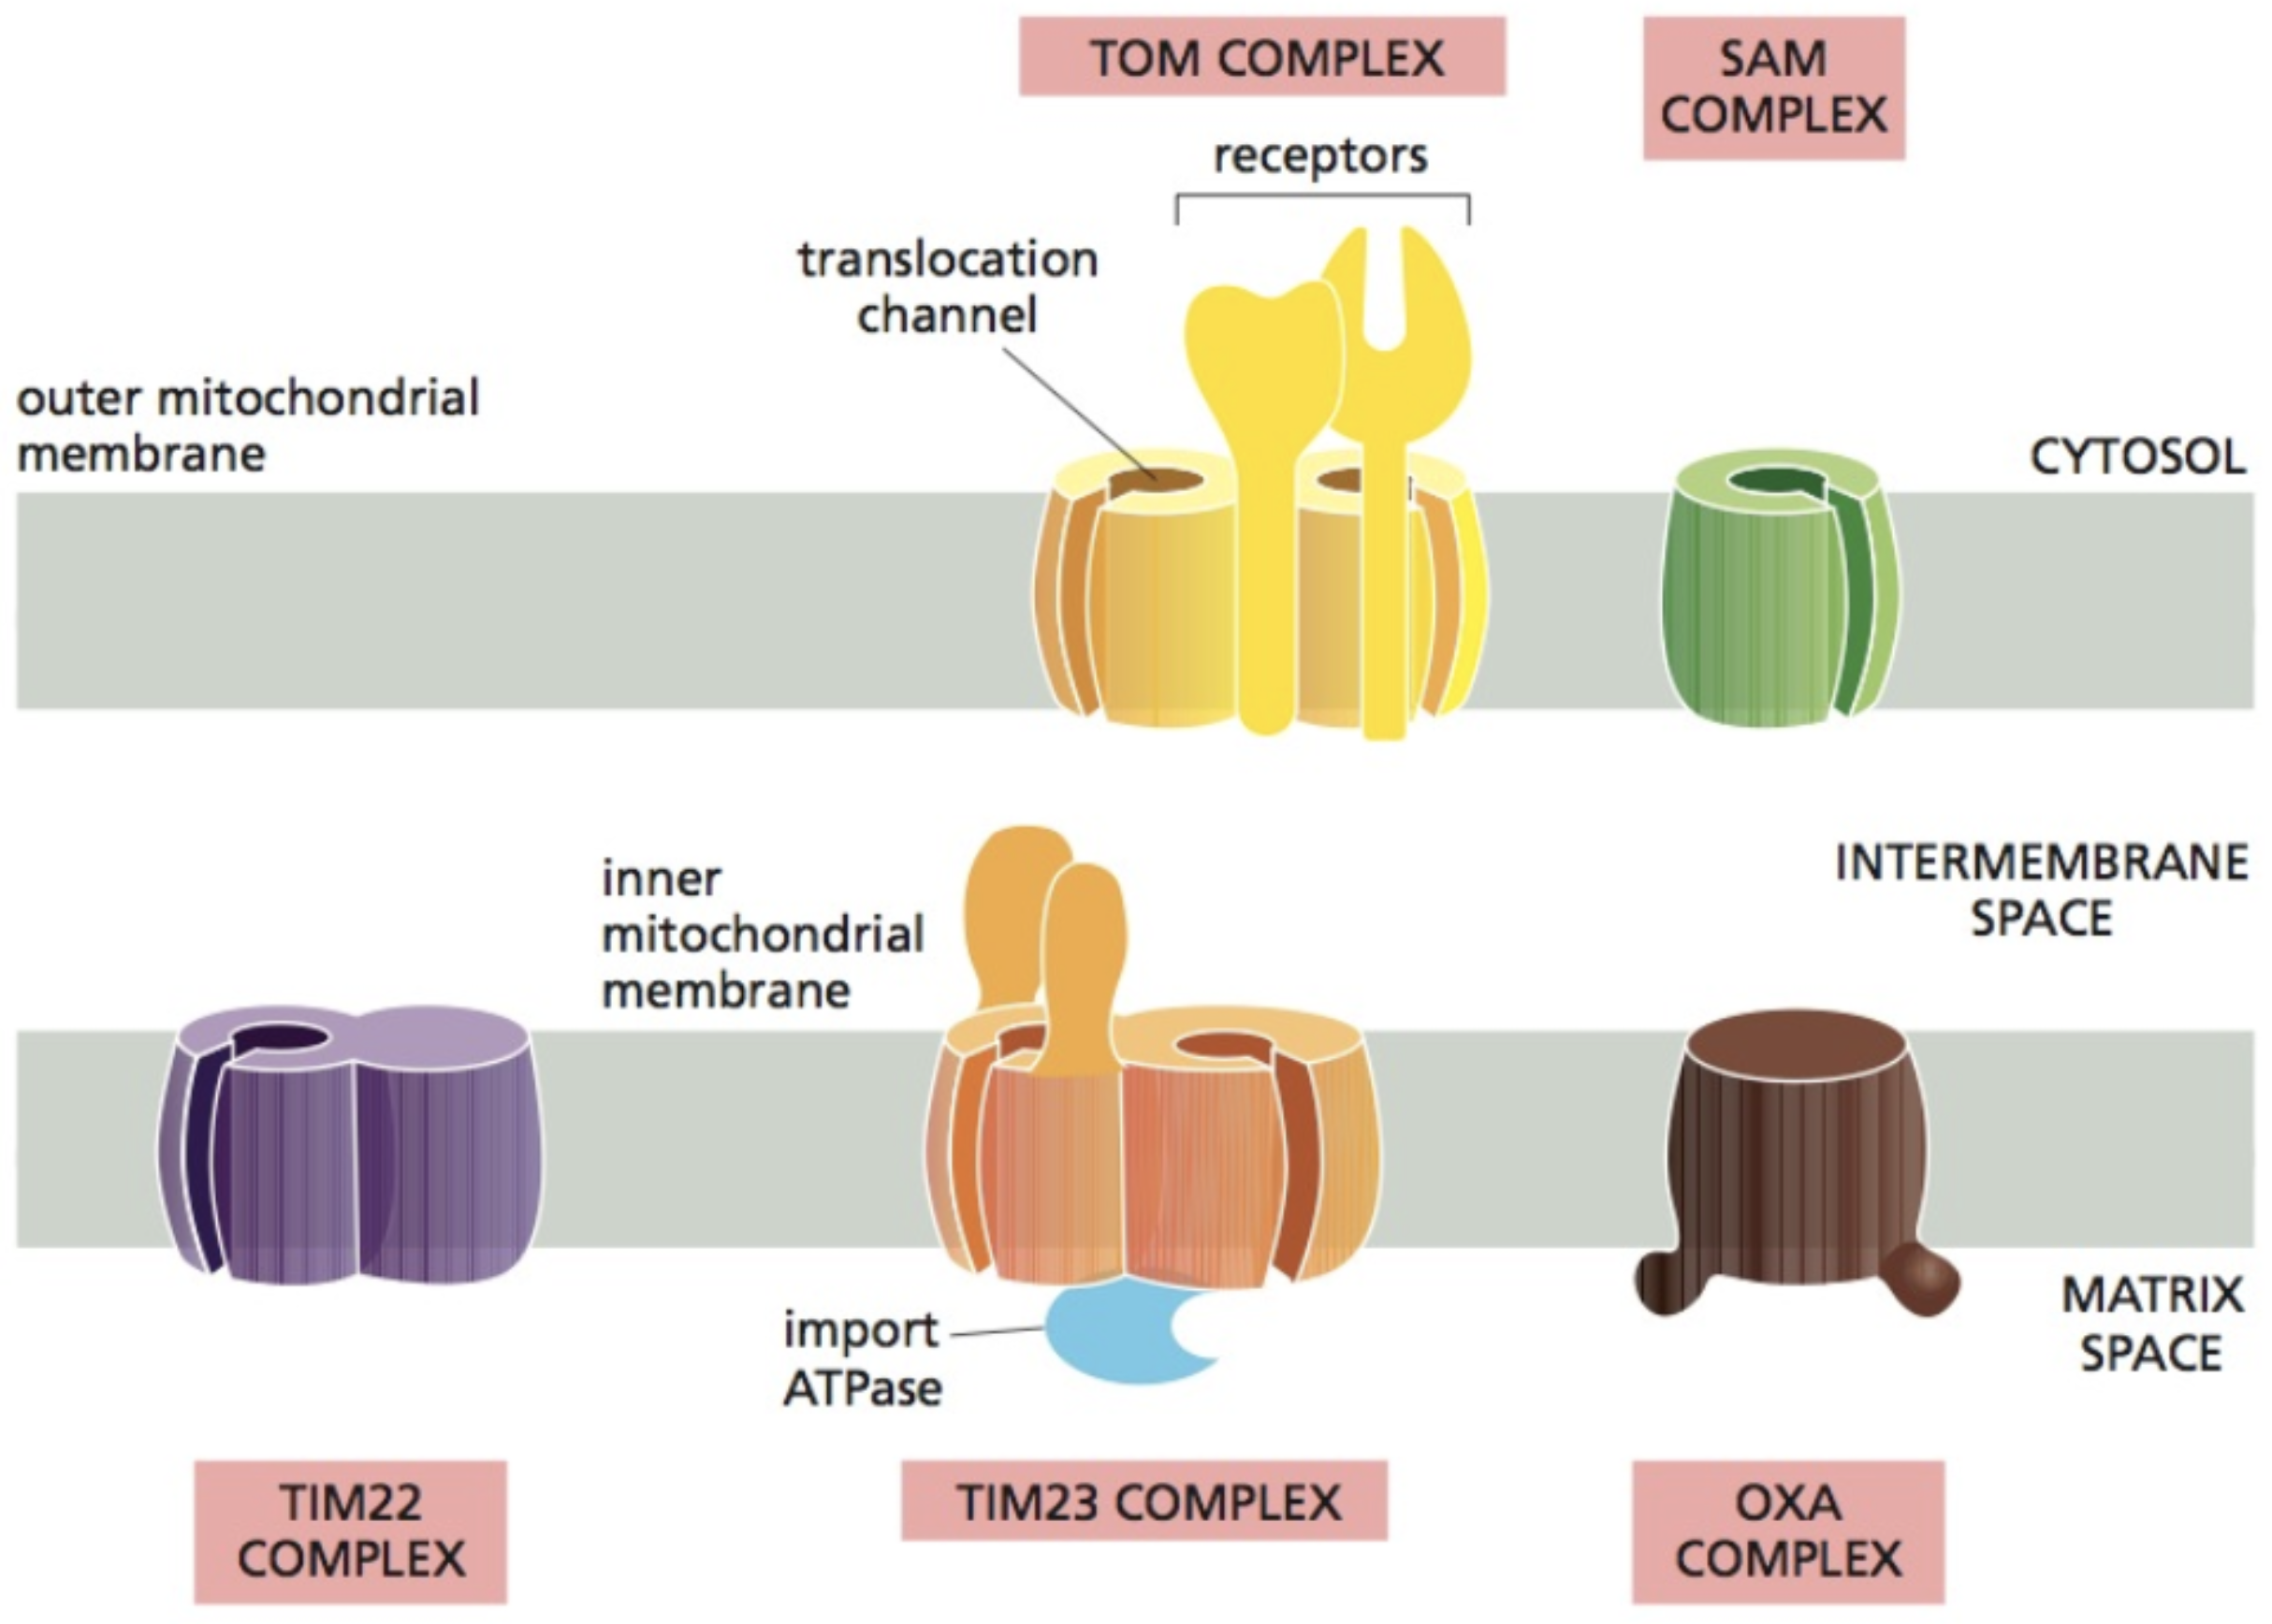
\includegraphics[width=0.5\linewidth]{../ExtFiles/MiTranslocators.png}
        \caption{Mitochondrial translocators.}
        \label{fig:MiTranslocators}
    \end{figure}
    \begin{itemize}
        \item These are all big, multiprotein complexes assembled on the various membranes.
    \end{itemize}
    \item \textbf{TOM complex}: The mitochondrial complex of proteins --- localized in the outer membrane --- responsible for the movement of proteins through this barrier and into the interluminal space. \emph{Also known as} \textbf{translocase of the outer membrane}.
    \item \textbf{TIM complex}: The mitochondrial complex of proteins --- localized in the inner membrane --- responsible for the movement of proteins through this barrier and into the matrix. \emph{Also known as} \textbf{translocase of the inner membrane}, \textbf{TIM23}.
    \item \textbf{SAM complex}: The mitochondrial complex of proteins --- localized in the outer membrane --- responsible for the folding/insertion of proteins into the outer membrane. \emph{Also known as} \textbf{sorting and assembly machinery complex}.
    \item \textbf{OXA complex}: The mitochondrial complex of proteins --- localized in the inner membrane --- responsible for the movement of proteins through this barrier and into the matrix. \emph{Also known as} \textbf{oxidase assembly complex}.
    \item There is a way to get TIM and TOM to lock together so translocation happens all at once from the cytosol to the matrix (instead of having to pass through the interluminal space).
    \begin{figure}[H]
        \centering
        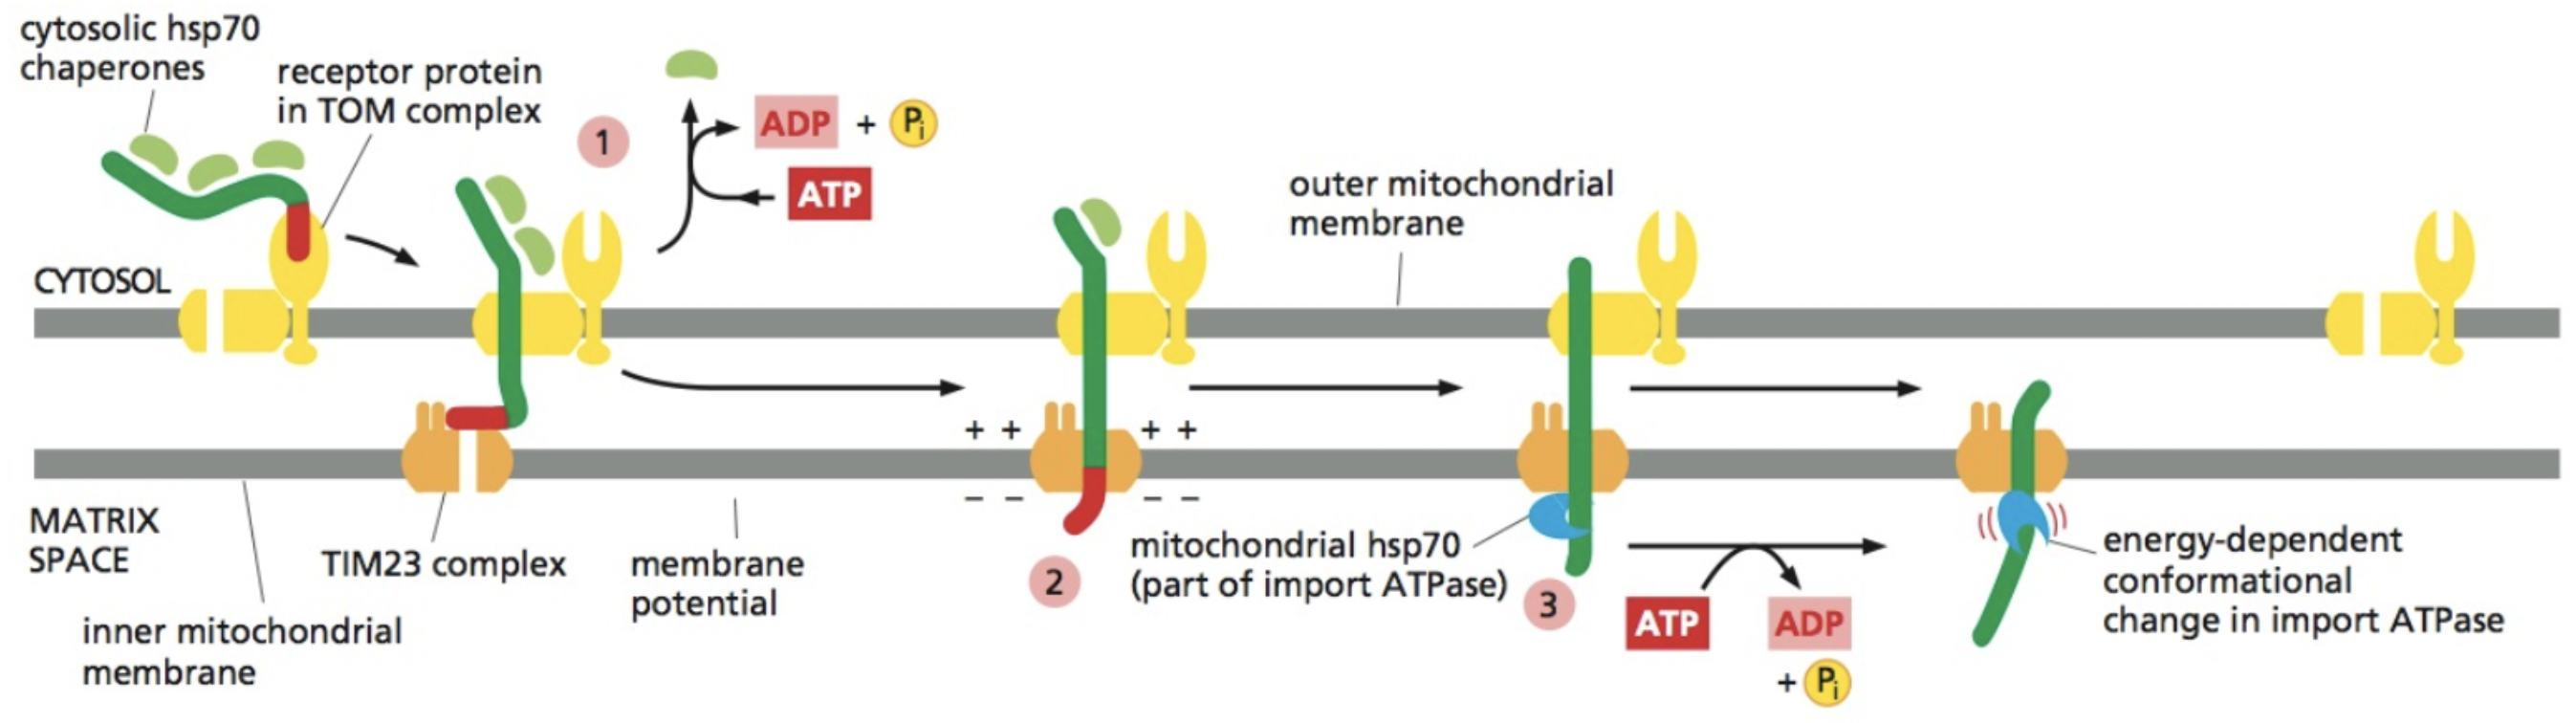
\includegraphics[width=0.97\linewidth]{../ExtFiles/MiTransCytMat.png}
        \caption{Translocation from the cytosol to the mitochondrial matrix.}
        \label{fig:MiTransCytMat}
    \end{figure}
    \begin{itemize}
        \item Role of energy in protein import into the mitochondrial matrix.
        \begin{itemize}
            \item Every ATP hydrolyzed at TOM causes you to pull the protein through by a couple of peptides.
            \item Membrane potential drives TIM.
        \end{itemize}
        \item Once the whole protein has been pulled through TOM, TOM and TIM separate.
        \item Once the translocation sequence has completely entered the matrix, a signal peptidase cleaves it, trapping the protein in the matrix.
    \end{itemize}
    \item We now talk about how proteins are sent to each membrane.
    \item Sending proteins to the outer membrane.
    \begin{figure}[h!]
        \centering
        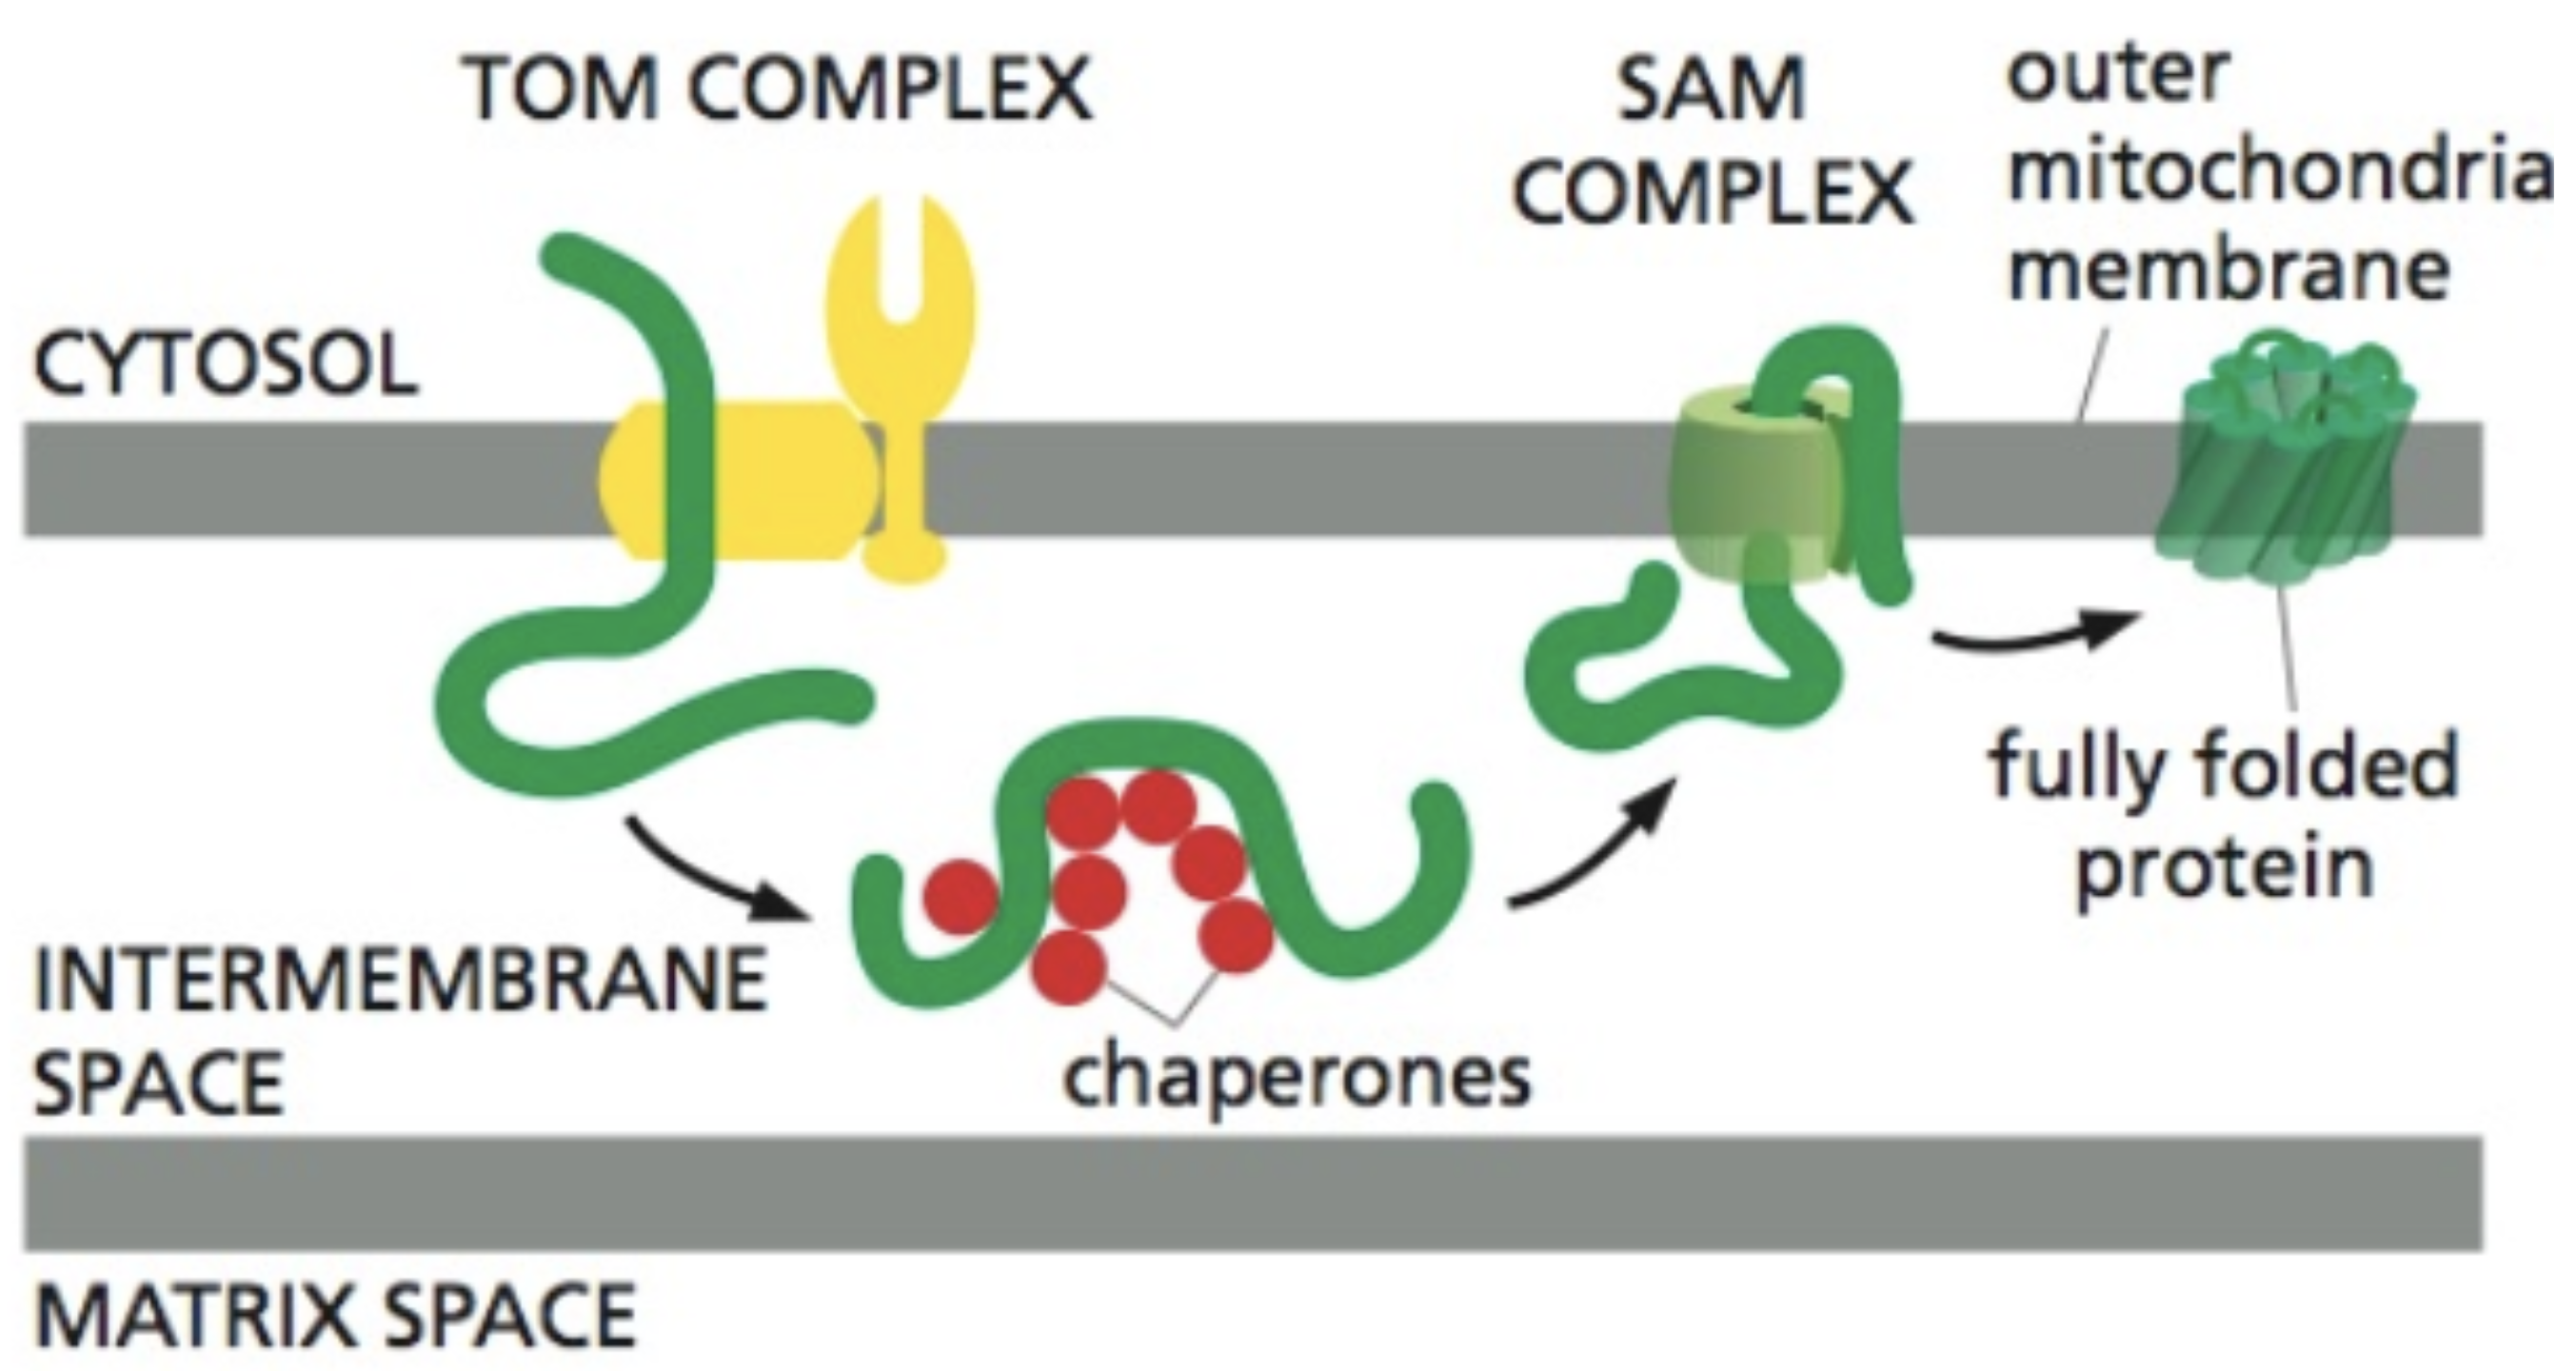
\includegraphics[width=0.35\linewidth]{../ExtFiles/MiTransCytOut.png}
        \caption{Translocation from the cytosol to the mitochondrial outer membrane.}
        \label{fig:MiTransCytOut}
    \end{figure}
    \begin{itemize}
        \item Many porins are present on the outer membrane.
        \item A protein first gets pulled into the interluminal space.
        \begin{itemize}
            \item Aside: In bacteria, this space is known as the \textbf{periplasm}.
            \item The periplasm is very nice for protein generation because there are very few proteins there and once you clone proteins there, all you have to do to release them is crack open the cell wall.
        \end{itemize}
        \item When proteins get pulled into the intermembrane space, they are all hydrophobic (because they will reside in a phospholipid bilayer eventually). Thus, they are prone to agregation in their water-based media, but chaperones latch on to separate them. Once stabilized in the intermembrane space, the protein then gets sent to SAM which folds it into the membrane. SAM has a slit, so as it pulls peptides in, it ejects them out laterally into the membrane.
        \begin{itemize}
            \item Aside: In a bacteria, there is an analogous BAM complex.
            \item Implication: This process is conserved between bacteria and mitochondria, further supporting the endosymbiotic theory.
        \end{itemize}
    \end{itemize}
    \item Sending proteins to the inner membrane.
    \begin{figure}[H]
        \centering
        \begin{subfigure}[b]{0.4\linewidth}
            \centering
            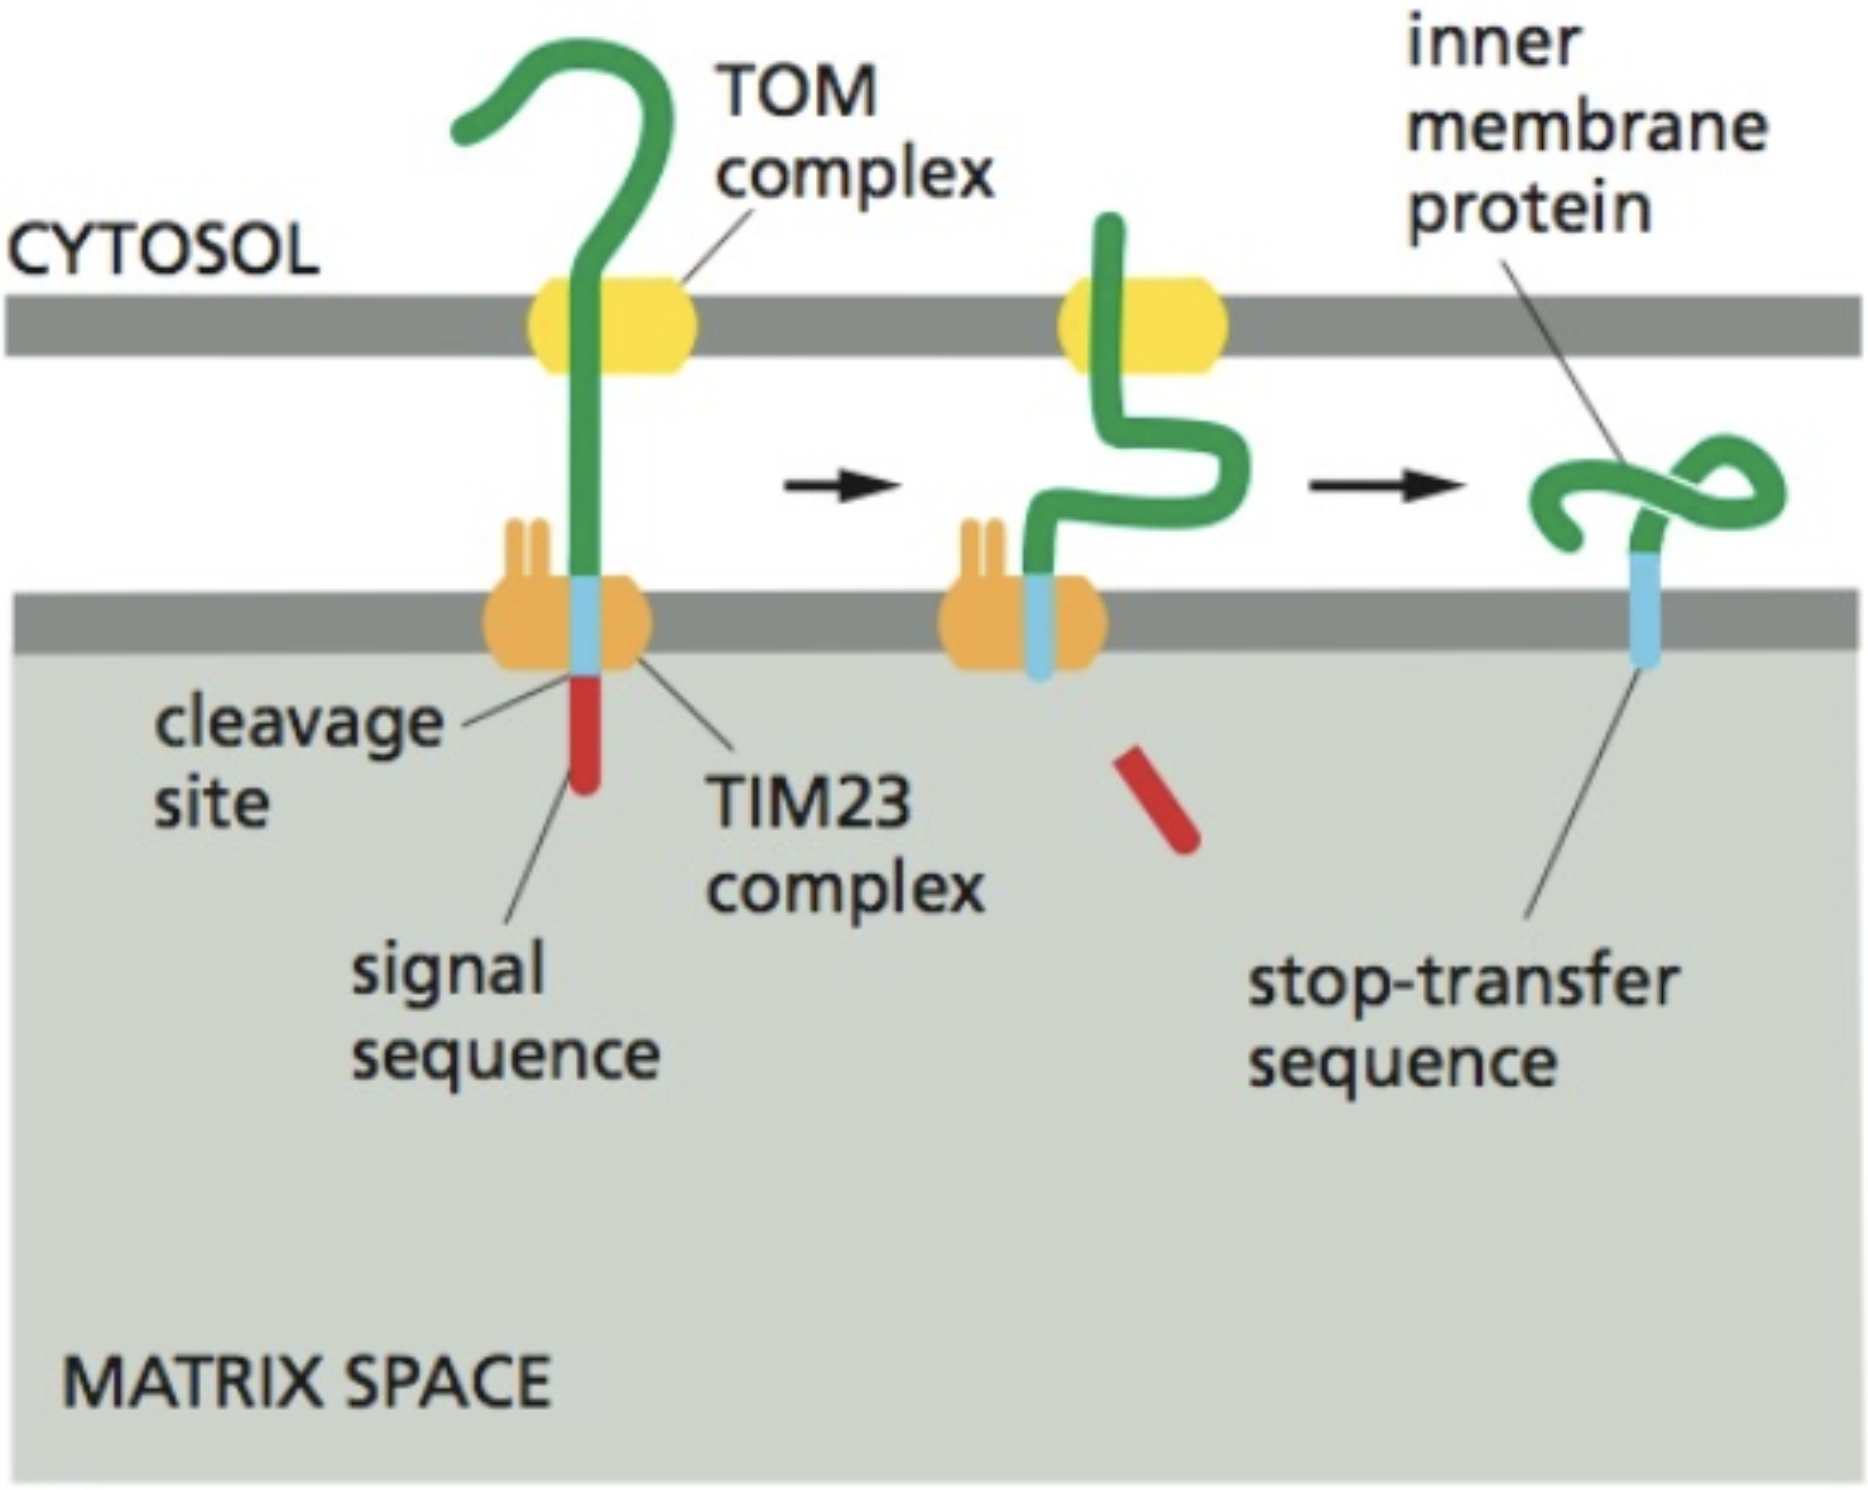
\includegraphics[width=0.8\linewidth]{../ExtFiles/MiTransCytIna.png}
            \caption{Direct insertion.}
            \label{fig:MiTransCytIna}
        \end{subfigure}
        \begin{subfigure}[b]{0.4\linewidth}
            \centering
            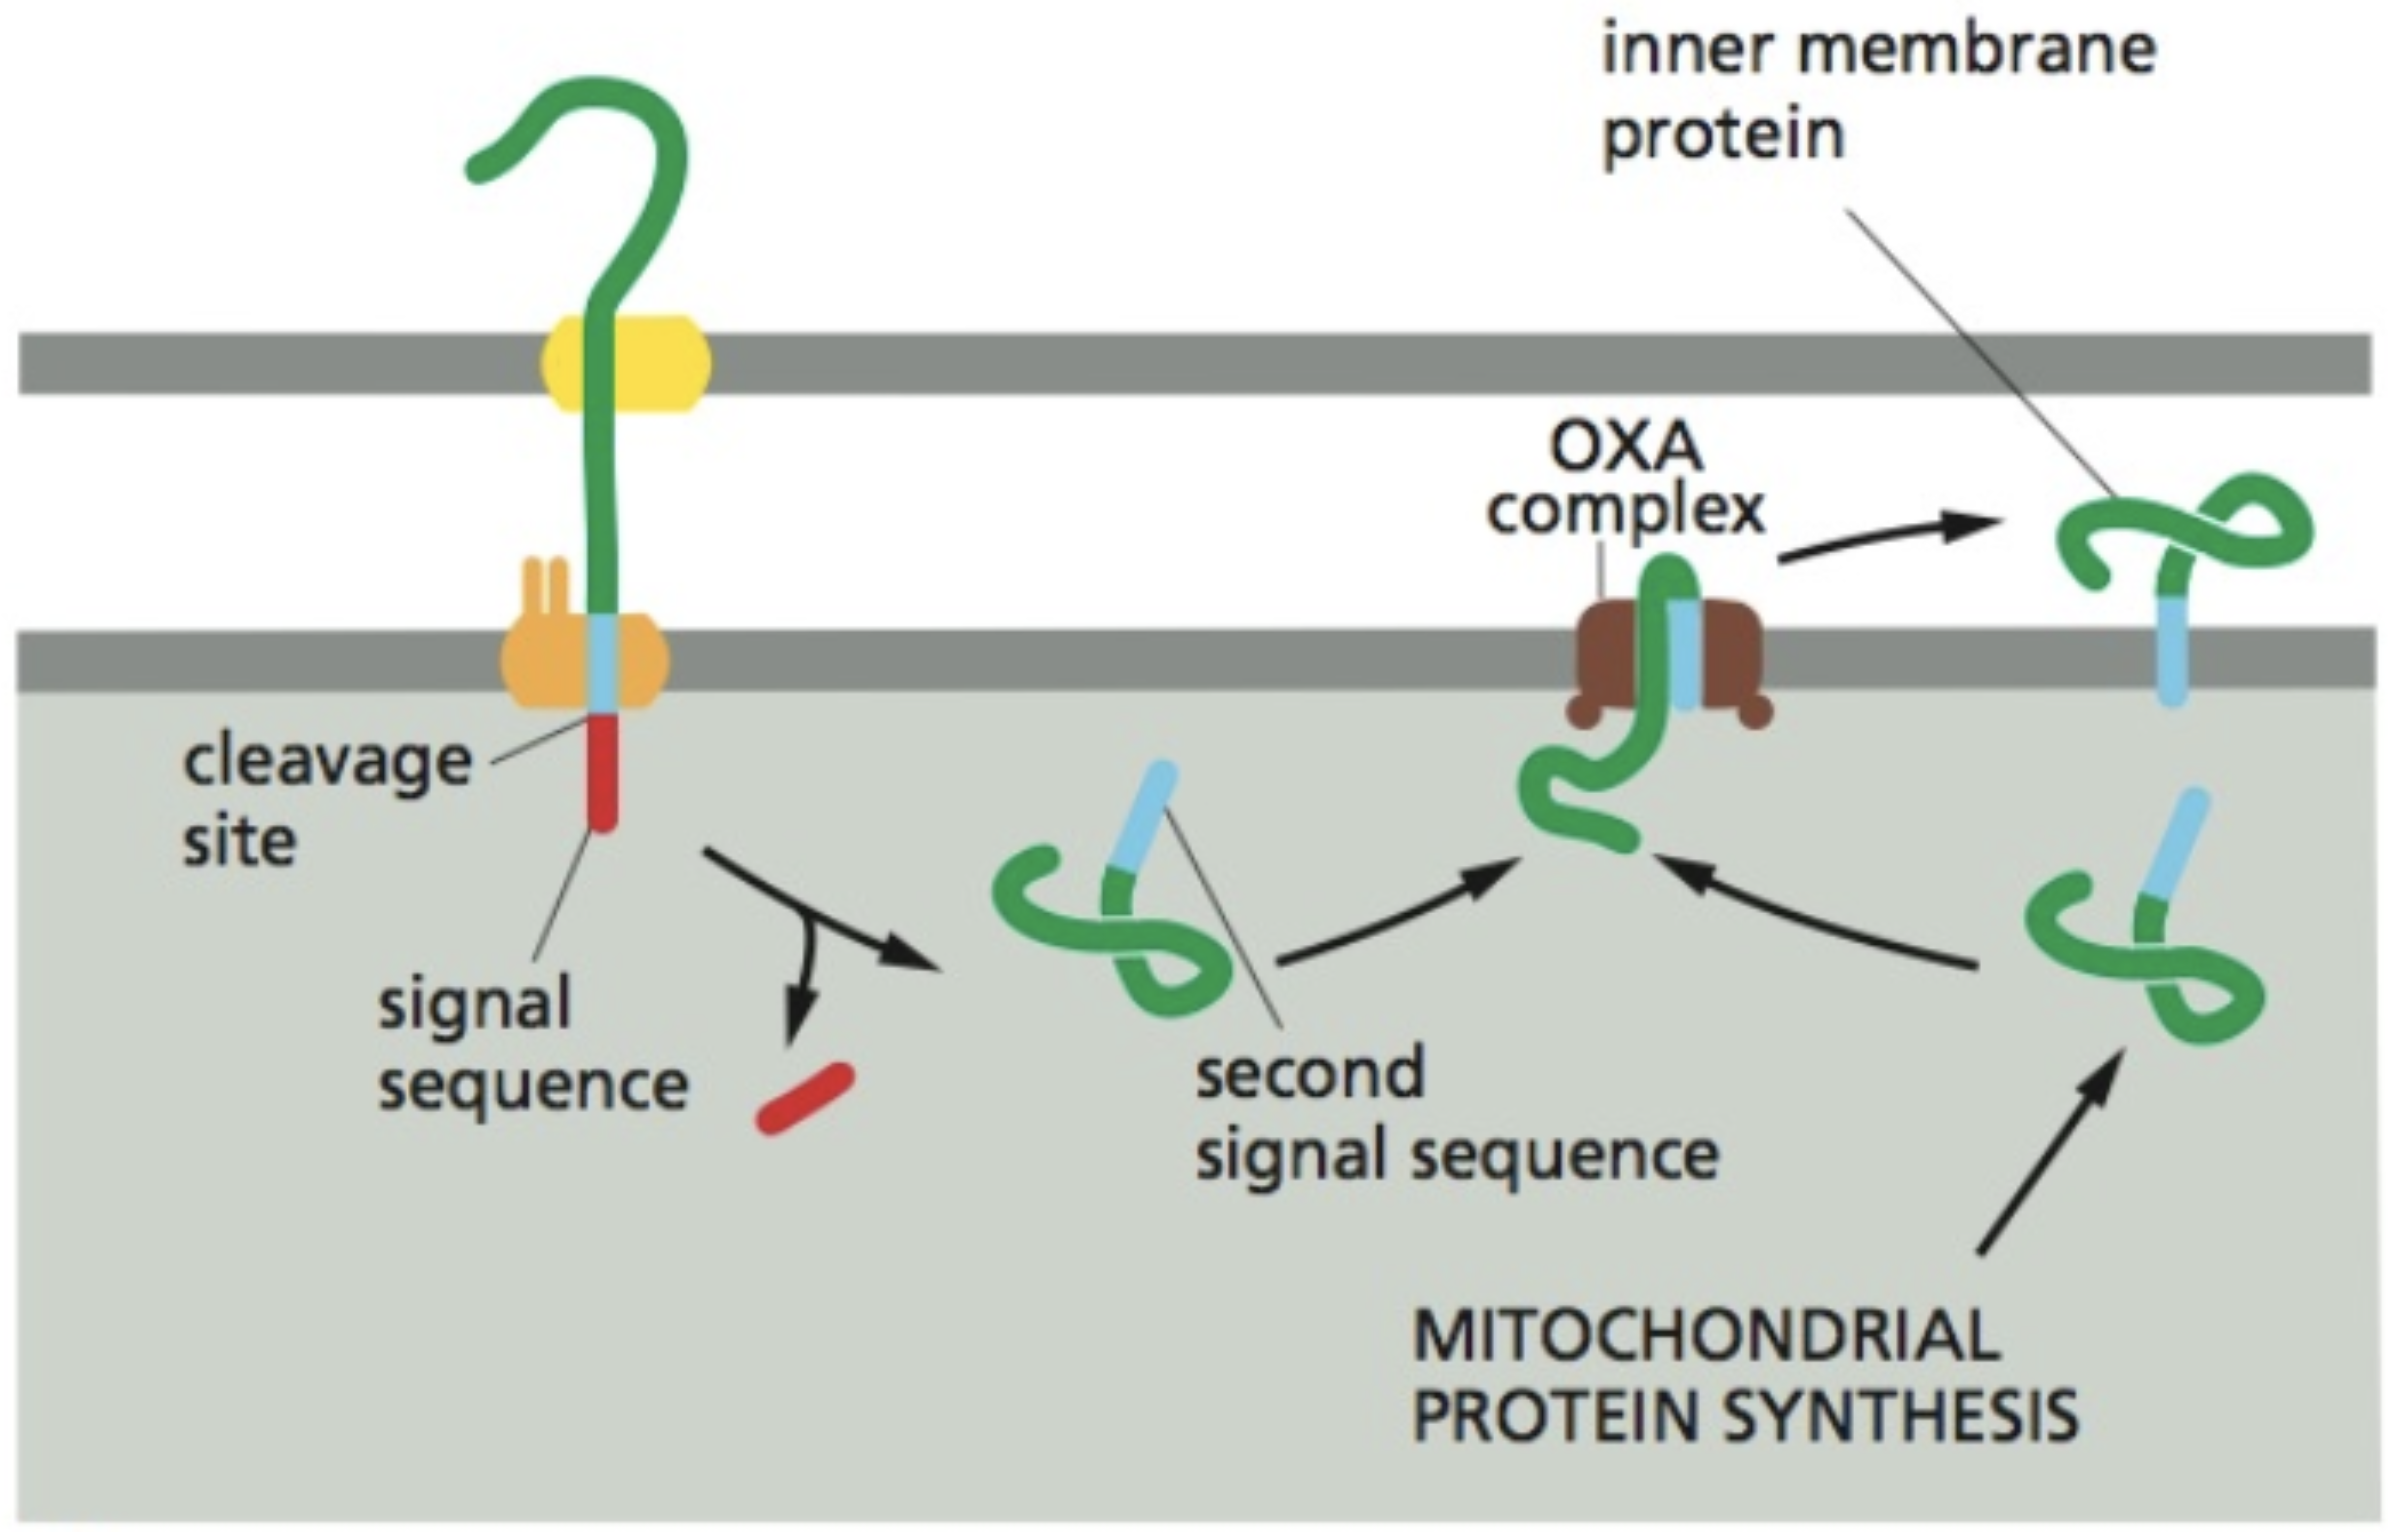
\includegraphics[width=0.98\linewidth]{../ExtFiles/MiTransCytInb.png}
            \caption{Via the OXA complex.}
            \label{fig:MiTransCytInb}
        \end{subfigure}\\[1em]
        \begin{subfigure}[b]{0.4\linewidth}
            \centering
            \includegraphics[width=0.85\linewidth]{../ExtFiles/MiTransCytInc.png}
            \caption{Multipass proteins.}
            \label{fig:MiTransCytInc}
        \end{subfigure}
        \caption{Translocation from the cytosol to the mitochondrial inner membrane.}
        \label{fig:MiTransCytIn}
    \end{figure}
    \begin{itemize}
        \item There are three methods by which this can occur.
        \item Method 1 (Figure \ref{fig:MiTransCytIna}).
        \begin{itemize}
            \item This method directly inserts single-pass transmembrane proteins into the inner membrane.
            \item Translocation begins as if the protein is to be pulled into the matrix, but immediately following the localization sequence, there is a stop-transfer sequence. When TIM interacts with this, it stops pulling the protein through, signal peptidase cleaves off the localization sequence, and TIM ejects the hydrophobic stop-transfer sequence into the inner membrane.
            \item Once TOM finishes pulling the bulk into the interluminal space and the protein refolds, we are done.
        \end{itemize}
        \item Method 2 (Figure \ref{fig:MiTransCytInb}).
        \begin{itemize}
            \item Use the OXA complex.
            \item The TIM/TOM complex moves a protein into the matrix and a single peptidase cleaves off the localization sequence.
            \item A secondary tag following the localization sequence then engages the OXA complex. The OXA complex flips the protein so that the tag is in the inner membrane and the bulk of the protein is in the interluminal space.
        \end{itemize}
        \item Method 3 (Figure \ref{fig:MiTransCytInc}).
        \begin{itemize}
            \item Multipass membrane proteins are introduced via the \textbf{TIM22 complex}.
        \end{itemize}
    \end{itemize}
    \item Import from the cytosol into the intermembrane space.
    \begin{figure}[H]
        \centering
        \begin{subfigure}[b]{\linewidth}
            \centering
            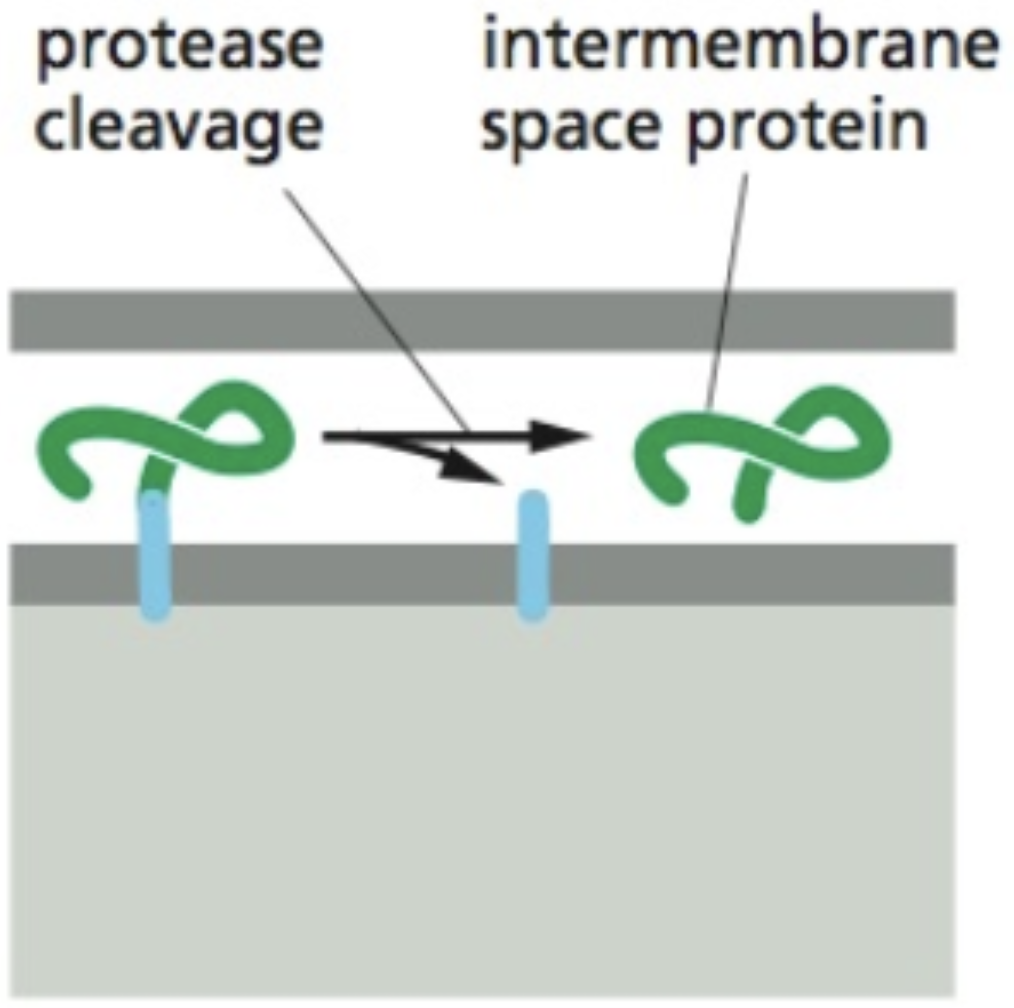
\includegraphics[width=0.15\linewidth]{../ExtFiles/MiTransCytLuma.png}
            \caption{Inner membrane cleavage.}
            \label{fig:MiTransCytLuma}
        \end{subfigure}
    \end{figure}
    \begin{figure}[h!]
        \ContinuedFloat
        \centering
        \begin{subfigure}[b]{\linewidth}
            \centering
            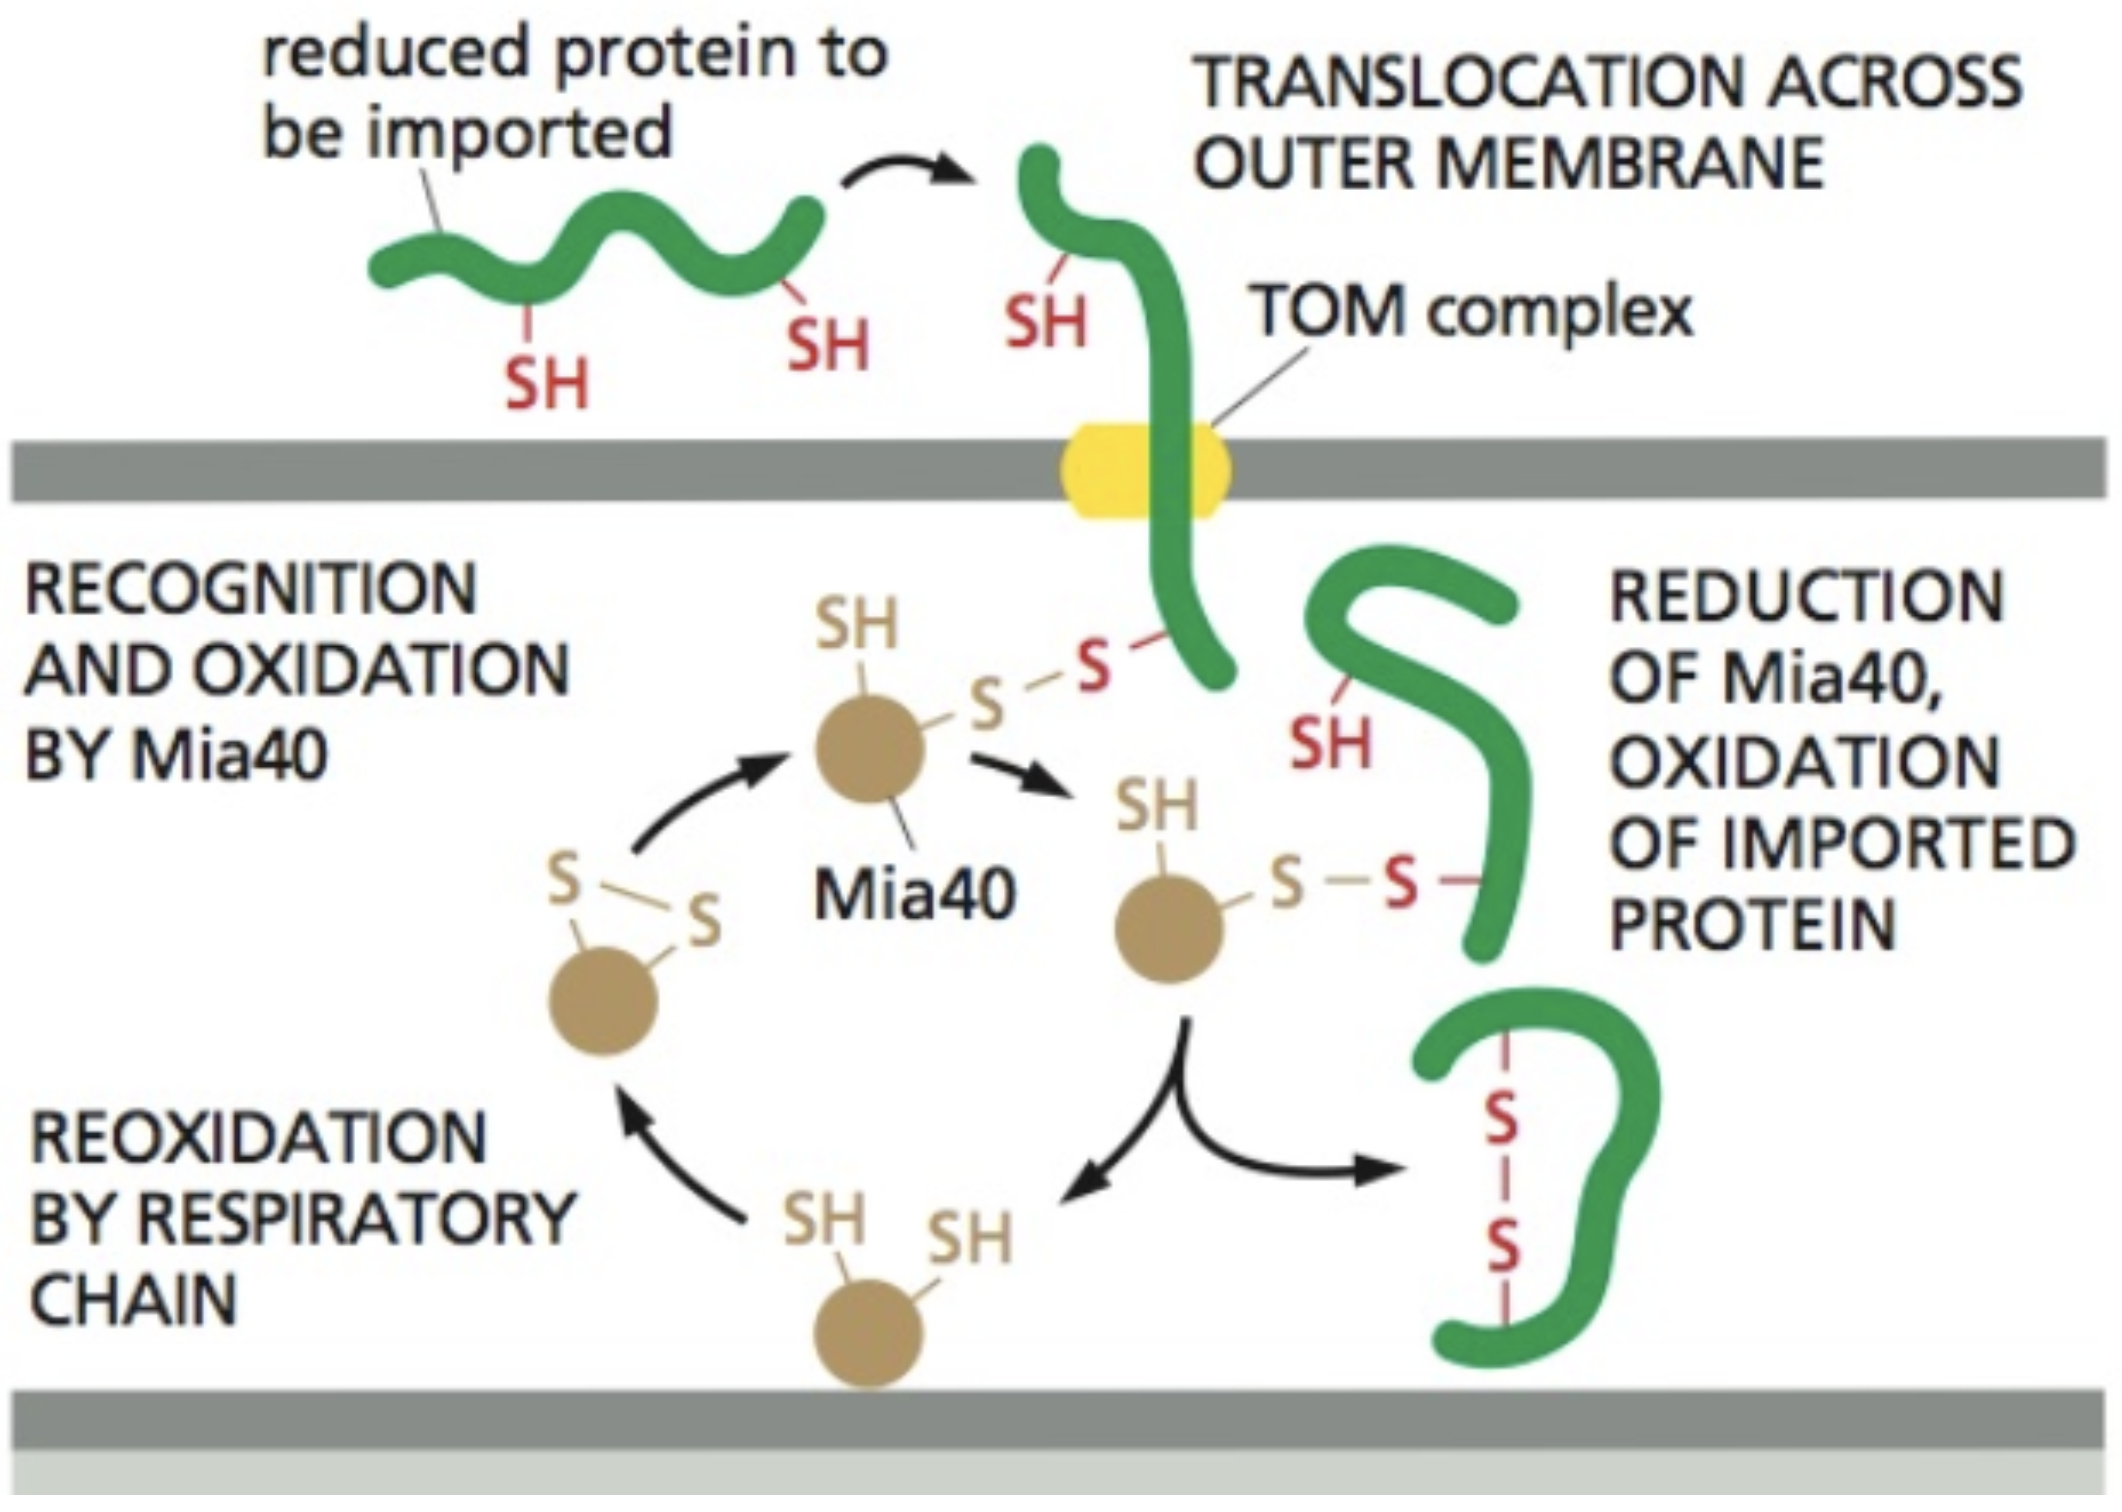
\includegraphics[width=0.38\linewidth]{../ExtFiles/MiTransCytLumb.png}
            \caption{Via Mia40.}
            \label{fig:MiTransCytLumb}
        \end{subfigure}
        \caption{Translocation from the cytosol to the mitochondrial interluminal space.}
        \label{fig:MiTransCytLum}
    \end{figure}
    \begin{itemize}
        \item If after insertion into the inner membrane, the bulk is cleaved from the transmembrane region, it will float away in the interluminal space. This is a secondary mechanism by which proteins enter the interluminal space, in addition to direct import by TOM.
        \item A third (and very popular) mechanism leverages disulfide bonds. These help the protein fold, but if the protein is to be pulled through TOM, these will have been reduced to split them and unfold the protein. When the reduced disulfide bonds interact with \textbf{Mia40} in the interluminal space, they get reassembled and Mia40 gets regenerated (it is a catalyst). This refolding sticks the protein in place.
    \end{itemize}
    \item Next time: Molecular mechanism of translocases; how they release transmembrane domains in the right origin.
    \item Peroxisomes.
    \begin{itemize}
        \item We understand very little about their function, but if anything is wrong with them, it's deadly.
        \item Take long lipid chains and cut them into shorter lipid chains by peroxidizing them (they have many reactive oxygen species).
        \item Smallest organelle in the cell (\SIrange{50}{100}{\nano\meter}) and has a very small number of proteins.
        \item Peroxisomes are thought to be born from the ER via budding. Then the peroxisome must mature and acquire proteins, both in its membrane and in the lumen.
        \item There are peroxisome targeting sequences, but who takes proteins to the peroxisomes and how they are transferred into the peroxisome is not clear.
        \item Peroxisomes are thought to undergo fission for replication, but we have no way to distinguish early peroxisomes from mature, functional ones.
        \item Peroxisomes carry their own catalase (which reduces oxygen into water and ROSs).
    \end{itemize}
    \item Summary of today.
    \begin{itemize}
        \item How compartments evolved; the evolution determines what is topologically equivalent to what. Nucleus and cytosol are equivalent (transport is facilitated by import and export factors), but most organelles are topologically equivalent to the extracellular matrix. You can take proteins to the nucleus or cytosol once they're born or to the mitochondria, or to specific places in the mitochondria.
    \end{itemize}
    \item Chemists are the best inventers, but they don't have a very good understanding of cell biology.
    \item GTPs are used for big conformational changes.
    \begin{itemize}
        \item The energy from hydrolyzing GTP and ATP is the same; it's just a question of how you use it molecularly.
    \end{itemize}
    \item Yamuna is very knowledgable about a variety of topics in her field.
\end{itemize}




\end{document}